%%%%%%%%%%%%%%%%%%%
%%%%%%%%%%%%%%%%%%%
%%%%%%%%%%%%%%%%%%%
%%%%%%%%%%%%%%%%%%%
\chapter{serie}

Data una successione $a_n$ di numeri reali o complessi
possiamo considerare la successione
delle cosiddette \myemph{somme!parziali}
\[
  S_n = \sum_{k=0}^{n} a_k.
\]
Potremo scrivere più concisamente $S_n = \sum a_n$.
Intuitivamente si intende sommare i termini della successione $a_k$
per $k$ che parte da $0$ fino a $k=n$:
\[
  \sum_{k=0}^n a_k = a_0 + a_1 + a_2 + \dots + a_n.
\]
Formalmente la somma $S_n=\displaystyle \sum_{k=0}^n a_k$
è definita ricorsivamente
dalle seguenti relazioni:
\[
  \begin{cases}
    S_0 = a_0, \\
    S_{n+1} = S_n + a_{n+1}.
  \end{cases}
\]

I numeri $a_n$ si chiamano \myemph{termini} della serie.
\index{termini!di una serie}\index{serie!termini}%
Se la successione delle somme parziali ammette limite il limite viene chiamato
\myemph{somma}
\index{somma!di una serie}\index{serie!somma}%
della serie e si indica con
\[
  \sum_{k=0}^{+\infty} a_k = \lim_{n\to +\infty} S_n = \lim_{n\to+\infty} \sum_{k=0}^n a_k.
\]

La terminologia già introdotta per le successioni si applica anche alle
serie che sono in effetti anch'esse delle successioni.
In particolare una serie può essere convergente, divergente o indeterminata.
Questo è il \emph{carattere della serie}.
\mynote{carattere}%
\index{carattere!di una serie}%
\index{serie!carattere}%

Più in generale si potrà considerare la somma che parte da un certo
indice $m\in \ZZ$.
Fissato $m$ si potrà ad esempio considerare la serie:
\[
  S_n = \sum_{k=m}^n a_k
\]
che risulta definita per ogni $n\in\NN$, $n\ge m$
come
\[
  S_n = a_m + a_{m+1} + \dots + a_n.
\]

\begin{example}
Consideriamo la serie $S_n$ definita
come la somma dei numeri naturali da $1$ a $n$:
\[
  S_n = \sum_{k=1}^n k = 1 + 2 + \dots + n.
\]
Si può dimostrare facilmente per induzione che si ha
\[
  S_n = \frac{n(n+1)}{2}.
\]
E mediante la definizione di limite si può verificare che
risulta $S_n \to +\infty$.

Questo si esprime dicendo che la serie $\sum n$ è divergente:
\[
     \sum_{k=1}^{+\infty} k = +\infty.
\]
\end{example}

\begin{example}[la serie geometrica]
Fissato $q \in \RR$ o $q\in \CC$ alla successione
$  a_n = q^n$
di termini
\[
  a_0 = 1,\qquad
  a_1 = q,\qquad
  a_2 = q^2,\qquad
  a_3 = q^3, \dots
\]
è associata la
\emph{serie geometrica}%
\mynote{serie geometrica}%
\index{serie!geometrica}
$\sum q^n$
le cui somme parziali sono
\[
  S_0 = 1, \qquad
  S_1 = 1 + q, \qquad
  S_2 = 1 + q + q^2, \qquad
  \dots
\]
\end{example}

Il seguente teorema ci mostra come per diversi valori di $q$
la serie geometrica assume
tutti i possibili caratteri:
convergente, divergente, indeterminato.

\begin{theorem}[somma della serie geometrica]
\mymark{***}
\mymargin{somma!della serie geometrica}
Sia $q\in \CC$. Se $q\neq 1$ si ha
\[
 \sum_{k=0}^n q^k  = \frac{1-q^{n+1}\!\!\!\!\!\!}{1-q}.
\]
Se $\abs{q} < 1$ la serie geometrica converge:
\[
 \sum_{k=0}^{+\infty} q^k = \frac{1}{1-q}.
\]

Se $\abs{q}\ge 1$ la serie non converge
ma dobbiamo distinguere se la serie
si considera a valori reali o complessi
per determinarne il carattere.

Se consideriamo la serie a valori reali
(quindi $q\in \RR$) se $q\ge 1$ la serie
diverge a $+\infty$,
se $q\le -1$ la serie è indeterminata.

Se consideriamo la serie a valori complessi
$q\in \CC$, se $\abs{q}>1$ la serie diverge
a $\infty$, lo stesso succede se $q=1$.
Se $\abs{q}=1$ ma $q\neq 1$ la serie
è indeterminata.
\end{theorem}
%
\begin{proof}
Il primo risultato riguarda una somma finita.
Si ha
\[
  (1-q)\cdot \sum_{k=0}^n q^k
  = \sum_{k=0}^n q^k - q \cdot \sum_{k=0}^n q^k
  = \sum_{k=0}^n q^k - \sum_{k=1}^{n+1} q^k
  = 1 - q^{n+1}
\]
da cui si ottiene, se $q\neq 1$, il risultato voluto.

Passando al limite per $n\to +\infty$, se $\abs{q} < 1 $
si nota che $\abs{q^{n+1}} = \abs{q}^{n+1} \to 0$
e la serie converge a $\frac 1{1-q}$.

Consideriamo ora la serie a valori reali.
Se $q>1$ osserviamo che
$q^n\to +\infty$ e quindi la serie diverge a $+\infty$
(infatti in questo caso $1-q$ è negativo).
Se $q=1$ si ha $q^k=1$ e quindi
$\displaystyle\sum_{k=0}^n q^k = n+1 \to +\infty$.

Per gli altri casi osserviamo che si ha
\[
  \sum_{k=0}^n q^k = \frac{1-q^{k+1}}{1-q}
  = \frac{1}{1-q} - \frac{q}{1-q}\cdot q^k
\]
e dunque il carattere della serie coincide
con il carattere della successione $q^k$.
Se consideriamo la successione a valori
complessi e se $\abs{q}>1$ la serie è divergente
a $\infty$ in quanto
$\abs{q^k}=\abs{q}^k\to +\infty$.
Se invece consideriamo la serie a valori reali
e $q<1$ (il caso $q\ge 1$ l'abbiamo già considerato)
la serie risulta indeterminata in quanto
in valore assoluto tende a $+\infty$ ma
il segno dei termini pari è opposto al segno dei termini
dispari.

Ci rimane da considerare il caso $\abs{q}=1$, $q\neq 1$.
Se $q$ è reale c'è solo il caso $q=-1$ e sappiamo
che $(-1)^k$ è indeterminata.
Anche se $q$ è complesso vogliamo dimostrare
che la successione $q^k$ è indeterminata:
se non lo fosse si avrebbe $q^k\to \ell$
con $\abs{\ell}=1$ in quanto $\abs{q^k}=1$.
e passando al limite nell'uguaglianza
\[
  q^{k+2} = q\cdot q^{k+1}
\]
si avrebbe $\ell = q\cdot \ell$ da cui
(dividendo per $\ell$) otteniamo $q=1$.
Dunque se $q\neq 1$ la successione $q^k$
è indeterminata e così è la serie
geometrica.
\end{proof}

\begin{theorem}[linearità della somma]
\mymargin{linearità della somma infinita}
Se $\sum a_n$ e $\sum b_n$ sono convergenti
allora per ogni $\lambda,\mu\in \CC$
anche $\sum (\lambda a_n + \mu b_n)$ è convergente
e si h
\[
 \sum_{k=0}^{+\infty} (\lambda a_n + \mu b_n)
 = \lambda \sum_{k=0}^{+\infty} a_n  + \mu \sum_{k=0}^{+\infty} b_n.
\]
\end{theorem}
%
\begin{proof}
Se $S_n$ e $R_n$ sono le somme parziali delle serie $\sum a_n$ e $\sum b_n$
allora le somme parziali della serie $\sum (\lambda a_n + \mu b_n)$ sono
$\lambda S_n + \mu R_n$ (in quanto sulle somme finite vale la proprietà distributiva e commutativa). Ma se $S_n \to S$ e $R_n \to R$ allora
$\lambda S_n + \mu R_n \to \lambda S + \mu R$.
\end{proof}

Osserviamo che le serie (così come le successioni) formano uno spazio
vettoriale in cui le operazioni di somma e prodotto per scalare vengono
eseguite termine a termine: $\sum a_n + \sum b_n = \sum (a_n + b_n)$,
$\lambda \sum a_n = \sum (\lambda a_n)$.
Il teorema precedente ci dice allora che le serie (così come le successioni)
convergenti sono un sottospazio vettoriale e che la somma della serie (così come il limite della successione) è un'operatore lineare definito su tale sottospazio.

\begin{theorem}[condizione necessaria per la convergenza]
\mymark{***}
\mymargin{condizione necessaria per la convergenza}
Se la serie $\sum a_n$ converge allora $a_n \to 0$.
\end{theorem}
%
\begin{proof}
\mymark{***}
Se la serie $\sum a_n$ converge significa che le somme parziali
$S_n = \sum_{k=0}^n a_k$ convergono: $S_n \to S$. Ma allora
\[
  a_n = S_n - S_{n-1} \to S - S = 0.
\]
\end{proof}

\begin{theorem}[stabilità del carattere]%
\index{carattere!di una serie}%
\index{stabilità!del carattere}%
\index{serie!stabilità del carattere}%
\index{serie!che differiscono su un numero finito di termini}%
Se le due successioni $a_n$ e $b_n$ differiscono solo su un numero finito
\mynote{stabilità del carattere}%
di termini, allora le serie corrispondenti $\sum a_n$ e $\sum b_n$ hanno lo stesso carattere.
\end{theorem}
%
\begin{proof}
Se le successioni differiscono su un numero finito di termini significa
che esiste un $N\in \NN$ tale che per ogni $k>N$ si ha $a_k=b_k$.
Dunque se indichiamo con $S_n = \sum_{k=0}^n a_k$ e $R_n = \sum_{k=0}^n b_k$
le corrispondenti successioni delle somme parziali, si avrà per ogni $n>N$
\[
  S_n - R_n
    = \sum_{k=0}^n a_k - \sum_{k=0}^n b_k
    = \sum_{k=0}^N (a_k - b_k) = C
\]
dove $C$ è una costante indipendente da $n$. Dunque
\[
  S_n = R_n + C.
\]
Se il limite di $R_n$ non esiste allora non esiste neanche il limite
di $S_n$ (altrimenti essendo $R_n = S_n -C$ anche il limite di $R_n$ dovrebbe esistere). Se il limite di $R_n$ è infinito allora il limite di $S_n$ è uguale
al limite di $R_n$. E se il limite di $R_n$ è finito anche il limite di $S_n$ è finito.

Dunque il carattere della successione $S_n$ è lo stesso della successione $R_n$
cioè le due serie hanno lo stesso carattere.
\end{proof}

Se una serie ha
primo termine con un indice diverso da $0$
ci si potrà sempre ricondurre (con un cambio di variabile)
ad una serie il cui indice parte da zero. Ad esempio
(facendo il cambio di variabile $j=k-1$ da cui $j=0$ quando $k=1$
e ricordando che l'indice utilizzato nelle somme delle
serie è una variabile muta):
\[
 \sum_{k=1}^{+\infty} \frac{1}{2^k}
 = \sum_{j=0}^{+\infty} \frac{1}{2^{j+1}}
 = \sum_{k=0}^{+\infty} \frac{1}{2^{k+1}}.
\]

Si osservi inoltre che in base al teorema precedente quale sia il primo indice
da cui si comincia a sommare non è rilevante per quanto riguarda il carattere della serie.
Se però la serie è convergente la sua somma può variare, ad esempio:
\[
 \sum_{k=1}^{+\infty} \frac{1}{2^k}
 = \enclose{\sum_{k=0}^{+\infty} \frac{1}{2^k}} - 2^0.
\]

Nota bene: in molti libri si scrive $\infty$ al posto di $+\infty$.
Risulta quindi molto comune omettere il segno $+$ davanti a $\infty$
nella terminologia delle serie (e anche delle successioni) visto
che gli indici si intendono numeri naturali e quindi $-\infty$ non avrebbe
senso.

Ci sono però casi in cui può essere utile usare anche gli indici negativi,
ad esempio
se $a_k$ è definita per ogni $k\in \ZZ$
si potrebbe definire (ma non lo faremo):
\[
  \sum_{k=-\infty}^{+\infty} a_k
  = \sum_{k=0}^{+\infty} a_k +
  \sum_{k=1}^{+\infty} a_{(-k)}
\]
richiedendo che entrambe le serie al lato destro
dell'uguaglianza esistano e non abbiano somme infinite di segno opposto.

\begin{theorem}[coda di una serie convergente]
\label{th:coda}
\mymark{*}
Sia $\sum a_n$ una serie convergente. Allora
\[
  \lim_{n\to +\infty} \sum_{k=n+1}^{+\infty} a_k = 0.
\]
\end{theorem}
%
\begin{proof}
\mymark{*}
Posto
\[
  S_n = \sum_{k=0}^n a_k,
\]
per definizione di serie convergente sappiamo che esiste $S$ finito
tale che $S_n \to S$. Osserviamo allora che
\[
  \sum_{k=n+1}^{+\infty} a_k = \lim_{N\to+\infty} \sum_{k=n+1}^N a_k
   = \lim_{N\to +\infty} S_N - S_n = S - S_n
\]
e, per $n\to +\infty$ si ha ovviamente $S - S_n \to S - S = 0$.
\end{proof}

\section{serie telescopiche}

Una serie scritta nella forma
% $\Sigma \Delta \vec a$ cioè
% del tipo:
\[
  \sum (a_{k} - a_{k+1})
\]
viene detta \emph{telescopica}
\mynote{serie telescopica}%
\index{serie!telescopica}
in quanto i singoli termini della somma (come i tubi di un cannocchiale),
si semplificano uno con l'altro (permettendo al cannocchiale di chiudersi):
\[
  S_n = \sum_{k=0}^n (a_{k} - a_{k+1})
  = \sum_{k=0}^{n} a_k - \sum_{k=1}^{n+1} a_k
  = a_0 - a_{n+1}.
\]

In linea teorica ogni serie può essere scritta in forma telescopica, basta infatti scegliere $a_0=0$, $a_n = -S_{n-1}$, affinché valga la relazione precedente. Scrivere una serie in forma telescopica è quindi equivalente a determinare la successione delle somme parziali.

\begin{example}[serie di Mengoli]
\mymark{**}
Si ha
\[
  \sum_{n=1}^{+\infty} \frac{1}{n(n+1)} = 1.
\]
\end{example}
%
\begin{proof}
\mymark{**}
Infatti
\[
  \sum_{k=1}^n \frac{1}{k(k+1)}
  = \sum_{k=1}^n \enclose{\frac{1}{k} - \frac{1}{k+1}}
  = \sum_{k=1}^n \frac{1}{k} - \sum_{k=2}^{n+1} \frac{1}{k}
  = 1 - \frac{1}{n+1} \to 1.
\]
\end{proof}

\section{serie a termini positivi}

\index{serie!a termini positivi}
Nel seguito considereremo serie i cui termini sono numeri reali
positivi (o almeno non negativi).
Quando scriveremo $a_n >0$ (o $a_n \ge 0$) sarà sempre
sottointeso che $a_n\in \RR$ visto che per i numeri complessi non
reali non abbiamo definito la relazione d'ordine.

\begin{theorem}[carattere delle serie a termini positivi]\label{th:serie_positiva}
\mymark{***}%
\mynote{carattere delle serie a termini positivi}%
\index{carattere!di una serie a termini positivi}%
Se $a_n\ge 0$
la serie $\sum a_n$ è regolare:
o converge oppure diverge a $+\infty$.
\end{theorem}
%
\begin{proof}
\mymark{***}
Se $a_n \ge 0$ essendo $a_n = S_n - S_{n-1}$ significa che
la successione $S_n$ delle somme parziali è crescente.
Dunque il limite delle $S_n$ esiste e non può essere negativo.
\end{proof}

\begin{theorem}[criterio del confronto]
\mymark{**}
\mynote{criterio del confronto}
\index{criterio!del confronto per serie}
Siano $\sum a_n$ e $\sum b_n$ serie a
termini positivi che si confrontano: $0\le a_n\le b_n$.
Allora
\[
  \sum_{k=0}^{+\infty} a_n \le \sum_{k=0}^{+\infty} b_n.
\]
In particolare se $\sum b_n$ converge anche $\sum a_n$ converge
e se $\sum a_n$ diverge anche $\sum b_n$ diverge.

Quest'ultimo risultato vale anche se $0 \le a_n \ll b_n$.
\end{theorem}
%
\begin{proof}
\mymark{*}
Se $S_n$ sono le somme parziali di $\sum a_n$ e $R_n$ sono le somme
parziali di $\sum b_n$ si ha $S_n \le R_n$ e il risultato
si riconduce al confronto tra successioni.

Nel caso in cui $a_n \ll b_n$ per definizione sappiamo che $\frac{a_n}{b_n}\to 0$
e quindi dalla definizione di limite sappiamo che
esiste $N$ tale che per ogni $n>N$ si ha (avendo scelto $\eps=1$)
\[
  \frac{a_n}{b_n} < 1.
\]
Dunque si ottiene $a_n \le b_n$ per tutti gli $n$ tranne al più un numero
finito. Sapendo che il carattere della serie non cambia se si modifica
la serie su un numero finito di termini ci si riconduce al caso precedente.
\end{proof}

\begin{example}\label{ex:52573}
\mymark{***}
La serie
\begin{equation}\label{eq:296453}
 \sum_{k=1}^{+\infty} \frac{1}{k^2}
\end{equation}
è convergente.
Infatti osservando che si ha per ogni $n>0$
\[
  \frac{1}{(n+1)^2} \le \frac{1}{n(n+1)}
\]
possiamo affermare che
\[
  \sum_{k=1}^{+\infty} \frac{1}{k^2}
  = 1 + \sum_{k=1}^{+\infty} \frac{1}{(k+1)^2}
  \le 1+ \sum_{k=1}^{+\infty} \frac{1}{k(k+1)}
  = 2
\]
in quanto ci siamo ricondotti alla
serie telescopica di Mengoli che ha somma pari a $1$.

Sappiamo quindi che la serie~\eqref{eq:296453} è convergente
senza sapere esattamente quale sia la sua somma.
Possiamo però trovare numericamente delle approssimazioni
della somma, facendo la somma dei primi termini
e stimando l'errore tramite la serie di Mengoli,
di cui sappiamo calcolare la somma.
Infatti se $S_N$ è la somma parziale dei primi
$N$ termini e $S = \lim S_N$ è la somma della serie,
essendo $1/(k+1)^2 \le 1/(k^2+k)$ si ha
\[
S_N
\le S
\le S_N + \sum_{k=N}^{+\infty} \frac{1}{k(k+1)}
\le S_N + \frac{1}{N}.
\]
Per calcolare le prime 6 cifre decimali esatte basterà
quindi sommare il primo milione di termini della serie.
Lo si può fare, ad esempio, con il codice riportato
a pagina~\pageref{code:series}, ottenendo $S=1.644934\ldots$

Utilizzando strumenti molto più avanzati
Eulero \index{Eulero}
(Leonard Euler, 1707--1783) è
riuscito ad esprimere la somma di questa serie mediante costanti matematiche fondamentali
(noi lo faremo con un metodo diverso nell'esercizio~\ref{ex:Basilea}).
\end{example}

\begin{corollary}[criterio del confronto asintotico]
\mymark{*}
\mynote{criterio del confronto asintotico}
\index{criterio!del confronto asintotico}
Se $a_n$ e $b_n$ sono successioni a termini positivi,
asintoticamente equivalenti (definizione~\ref{def:ordine_infinito}),
allora le serie corrispondenti $\sum a_n$ e $\sum b_n$
hanno lo stesso carattere.
\end{corollary}
%
\begin{proof}
\mymark{*}
Le serie a termini positivi non possono essere indeterminate
quindi è sufficiente verificare che se una serie converge, converge anche l'altra.
Essendo $a_n / b_n$ convergente tale rapporto deve anche essere
limitato, quindi esiste $C\in \RR$ tale che
\[
   a_n \le C \cdot b_n.
\]
Se la serie $\sum b_n$ converge anche $\sum C \cdot b_n$ converge e, per confronto,
converge anche $\sum a_n$.

Viceversa, scambiando il ruolo di $a_n$ e $b_n$ si verifica che se $a_n$
converge, converge anche $b_n$.
\end{proof}

\begin{example}
La serie
\[
\sum_n \frac{n^2+2n+3}{2n^4-n^3+n+1}
\]
è convergente. Infatti si può facilmente verificare che
\[
   \frac{n^2+2n+3}{2n^4-n^3+n+1} \sim \frac{1}{2n^2}.
\]
Ma sappiamo che la serie $\sum 1/n^2$ è convergente, di conseguenza
anche la serie $\sum 1/(2n^2)$ lo è (per linearità della somma)
e quindi, per confronto
asintotico, anche la serie data è convergente.
\end{example}

\begin{theorem}[criterio della radice]
\mynote{criterio della radice}
\index{criterio!della radice}
Sia $\sum a_n$ una serie a termini non negativi
(cioè $a_n\ge 0$) tale che
\mymark{***}
$\sqrt[n]{a_n} \to \ell \in [0,+\infty]$.
Se $\ell<1$ allora la serie converge.
Se $\ell>1$ allora la serie diverge.

Più in generale il risultato è valido con
\[
  \ell = \limsup \sqrt[n]{a_n}
\]
anche nel caso in cui il limite di $\sqrt[n]{a_n}$ non dovesse esistere.
\end{theorem}
%
\begin{proof}
\mymark{***}
Nel caso $\ell < 1$
prendiamo $q$ con $\ell < q < 1$ e poniamo $\eps = q-\ell$.
Per la definizione di limite $\sqrt[n]{a_n}\to \ell$
(ma basta che sia $\limsup \sqrt[n]{a_n}=\ell$)
sappiamo
esistere $N$ tale che per ogni $n > N$ si abbia
\[
  \sqrt[n]{a_n} < \ell + \eps = q
\]
cioè
\[
   a_n < q^n.
\]
Sapendo che $\sum q^n$ converge, sapendo anche che il carattere
della serie non cambia modificando un numero finito di termini,
per confronto possiamo concludere che anche la serie $\sum a_n$ converge.

Se $\ell>1$ si ha che $\sqrt[n]{a_n}>1$ e quindi $a_n>1$ per infiniti valori di $n$. La successione $a_n$ non è infinitesima e quindi la serie non può convergere.
\end{proof}

\begin{example}
La serie
\[
  \sum_k 2^{(\ln k) - k}
\]
è convergente. Infatti si ha
\[
 \sqrt[k]{2^{\ln k - k}}
 = 2^{\frac{\ln k - k}{k}}
 = 2^{\frac{\ln k }k - 1}
 \to 2^{-1}
 = \frac{1}{2}
 < 1.
\]
\end{example}

\begin{theorem}[criterio del rapporto]
\mymark{***}
\mynote{criterio del rapporto}
\index{criterio!del rapporto per serie}
Sia $\sum a_n$ una serie a termini non negativi
($a_n\ge 0$)
tale che $a_{n+1} / a_n \to \ell \in [0,+\infty]$.
Se $\ell <1$ allora la serie converge.
Se $\ell > 1$ la serie diverge.
\end{theorem}
%
\begin{proof}
\mymark{*}
Non sarebbe difficile fare una dimostrazione diretta, simile alla dimostrazione fatta per il criterio della radice.
Possiamo però osservare che
per il criterio di convergenza alla Cesàro (teorema~\ref{th:criterio_cesaro}) si ha $\sqrt[n]{a_n} \to \ell$
quindi ci riconduciamo al criterio della radice senza dover fare ulteriori dimostrazioni.
\end{proof}

\begin{example}
\mymark{***}
Per ogni $x\ge 0$ la serie
\[
  \sum \frac{x^n}{n!}
\]
converge.
\end{example}
%
\begin{proof}
Applichiamo il criterio del rapporto.
Posto $a_n = x^n / n!$ si ha
\[
\frac{a_{n+1}}{a_n}
= \frac{x^{n+1}}{(n+1)!}\cdot \frac{n!}{x^n}
= \frac{x}{n+1} \to 0 < 1.
\]
Dunque la serie converge.
\end{proof}

\subsection{associatività della somma di una serie}

\begin{example}
Posto $a_k = (-1)^k$ sappiamo che la serie corrispondente:
\[
  1 - 1 + 1 - 1 + 1 \dots
\]
è indeterminata perché le somme parziali sono
\[
  S_n = \sum_{k=0}^n (-1)^k
  = \begin{cases}
   1 & \text{se $n$ pari}\\
   0 & \text{se $n$ è dispari.}
  \end{cases}
\]
Se però associamo i termini a due a due otteniamo la serie
\[
  (1-1) + (1-1) + (1-1) \dots = 0 + 0 + 0 + \dots = 0
\]
che è convergente.
Il motivo è che la successione delle somme
parziali di questa nuova serie è una particolare estratta (quella
con gli indici pari) della successione delle somme parziali della
serie originale. Quindi non ci dovrebbe sorprendere il fatto che
nonostante la serie originale fosse indeterminata è possibile
associare i termini della serie in modo da ottenere una serie
regolare (in questo caso convergente).
In effetti per il teorema~\ref{th:bolzano_weierstrass} 
di Bolzano-Weierstrass sappiamo che
è sempre possibile estrarre una sottosuccessione regolare (convergente o divergente)
da qualunque successione.
Anche quando da una serie indeterminata si estrae una serie
convergente la somma della serie può dipendere da come i termini
vengono associati.
Se ad esempio nella serie precedente prendessimo
solamente le somme di indice dispari
otterremmo:
\[
  1 + (-1+1) + (-1+1) + \dots = 1.
\]
\end{example}

L'esempio precedente ci mostra che associando i termini di una
serie indeterminata è possibile ottenere serie con carattere
e somma diversi.
Il seguente teorema ci dice che questo fenomeno \emph{cattivo}
può solo avvenire quando si parte da una serie indeterminata.
Se la serie è regolare allora possiamo associarne i termini
senza modificarne né il carattere né la somma.
In particolare questo è vero per le serie a termini positivi.

\begin{theorem}[associatività delle serie regolari]%
\label{th:serie_associativa}%
Se $\sum a_k$ è una serie, scelta comunque
una successione crescente $k_n$ con $k_0=0$
possiamo considerare la serie $\sum b_n$
i cui termini
\[
  b_n = \sum_{j=k_n}^{k_{n+1}-1} a_j
\]
si ottengono associando i termini di $a_k$ a gruppi
consecutivi delimitati dalla successione di indici
$k_n$.

Se la serie $\sum a_k$ è regolare (convergente o divergente)
allora anche la serie $\sum b_n$ è regolare e si ha
\[
\sum_{n=0}^{+\infty} b_n
= \sum_{k=0}^{+\infty} a_k.
\]

In particolare questo vale se la serie $\sum a_k$ è a termini
positivi.
\end{theorem}
%
\begin{proof}
Siano $S_k = \sum_{j=0}^k a_j$ le somme parziali della
serie $\sum a_j$. Allora le somme parziali della serie $\sum b_n$
non sono altro che la sottosuccessione $S_{k_n}$.
Dunque se $S_k$ converge anche ogni sua sottosuccessione
converge allo stesso limite.

Il teorema~\ref{th:serie_positiva} ci dice
che le serie a termini positivi sono regolari e quindi
soddisfano le ipotesi del teorema.
\end{proof}

\subsection{la serie armonica}

Osserviamo che il criterio del rapporto non si applica alla
\emph{serie armonica}%
\mynote{serie armonica}%
\index{serie!armonica}%
\[
  \sum_k \frac{1}{k}
\]
in quanto
\[
 \frac{\frac{1}{k+1}}{\frac{1}{k}}
 = \frac{k}{k+1} \to 1.
\]

Per capire se la serie armonica converge o diverge presentiamo il metodo
di \emph{condensazione} che verrà enunciato in generale nel prossimo teorema
ma che può essere meglio compreso se applicato al caso particolare
della serie armonica.

Mostreremo che la serie armonica diverge.
L'idea è semplicemente quella di associare gli addendi della serie armonica
in gruppi di lunghezza potenze di due e stimare la somma di ogni gruppo dal basso
con il termine più piccolo (cioè l'ultimo) di ogni gruppo:
\begin{align*}
 \sum_{k=1}^{+\infty} \frac{1}{k}
 & = 1 + \frac 1 2
     + \enclose{\frac 1 3 + \frac 1 4}
     + \enclose{\frac 1 5 + \frac 1 6 + \frac 1 7 + \frac 1 8}
     + \dots\\
 & > 1 + \frac 1 2 + 2 \cdot \frac 1 4 + 4 \cdot \frac 1 8 + \dots \\
   & = 1 + \frac 1 2 + \frac 1 2 + \frac 1 2 + \dots
    = +\infty.
\end{align*}

\begin{theorem}[criterio di condensazione di Cauchy]%
\mymark{**}%
\mynote{criterio di condensazione di Cauchy}%
\index{criterio!di condensazione di Cauchy}%
Sia $a_n$ una successione decrescente di numeri reali non negativi:
$a_n \ge 0$.
Allora la serie $\sum a_k$ converge se e solo se converge
la serie
\[
  \sum 2^k a_{2^k}.
\]
\end{theorem}
%
\begin{proof}
\mymark{**}
Supponiamo per comodità che le somme partano da $k=1$.
Si tratta di raggruppare i termini $a_k$ in gruppi di potenze di due:
\begin{align*}
  b_0 & = a_1, \\
  b_1 &= a_2 +  a_3, \\
  b_2 &= a_4 +  a_5 +  a_6 +  a_7, \\
  b_3 &= a_8 +  a_9 +  a_{10} + \dots + a_{15}, \\
  &\vdots\\
  b_n &= a_{2^n} +  a_{2^{n}+1} + \dots + a_{2^{n+1}-1},\\
  &\vdots
\end{align*}
Grazie al teorema~\ref{th:serie_associativa} sulla associatività
delle serie a termini positivi sappiamo che
  \[
  \sum_{k=1}^{+\infty} a_k = \sum_{n=0}^{+\infty} b_n.
  \]
Ogni termine $b_n$ è la somma di $2^n$ termini della
successione $a_k$ che, essendo la successione decrescente,
possono essere stimati dall'alto e dal basso con il primo
e l'ultimo termine di ogni somma, dunque:
\[
  2^n a_{2^{n+1}-1} \le b_n \le 2^n a_{2^{n}}.
\]
Per ipotesi la serie $\sum 2^n a_{2^n}$ è convergente
dunque per confronto anche la serie $\sum b_n$ è convergente.

Viceversa se la serie $\sum 2^n a_{2^n}$ è divergente
anche la serie $\sum 2^{n+1} a_{2^{n+1}}$ è divergente
e sapendo che $b_n\ge 2^n a_{2^{n+1}-1}\ge \frac 1 2 2^{n+1} a_{2^{n+1}}$
otteniamo, per confronto, che anche la serie $\sum b_n$ è divergente.
\end{proof}

\begin{corollary}[serie armonica generalizzata]
\mymark{***}
\mynote{serie armonica generalizzata}%
\index{serie!armonica!generalizzata}
La serie
\[
 \sum_n \frac{1}{n^\alpha}
\]
converge se $\alpha>1$,
diverge se $0\le \alpha\le 1$.
\end{corollary}
%
\begin{proof}
\mymark{***}
Applichiamo il criterio di condensazione. Posto $a_n = \frac 1{n^\alpha}$ Si ha
\[
  \sum_n 2^n a_{2^n} = \sum_n 2^n \frac{1}{(2^n)^\alpha}
  = \sum_n 2^{n(1-\alpha)}
  = \sum_n \enclose{2^{(1-\alpha)}}^n
\]
che è una serie geometrica di ragione $q=2^{1-\alpha}$.
Se $\alpha>1$ allora $q<1$ e la serie armonica è convergente
se invece $\alpha \le 1$ allora $q\ge 1$ e la serie
armonica è divergente.
\end{proof}

\begin{exercise}
Utilizzare il criterio di condensazione per dimostrare che la serie
\[
  \sum \frac{1}{n \cdot \ln n}
\]
diverge.
\end{exercise}

\begin{exercise}
  Per quali valori dei parametri $\alpha\in \RR$ e $\beta\in \RR$
  la serie
  \[
    \sum n^\alpha (\ln n)^\beta
  \]
  converge?
\end{exercise}

%%%
%%%
\section{rappresentazione posizionale dei numeri reali}
%%%
%%%
Quando scriviamo $\frac{3}{8} = 0.375$ intendiamo che vale 
\[
\frac 3 8 = \frac{3}{10} + \frac{7}{10^2} + \frac{5}{10^3}.  
\]
Più in generale data una base $d\in \NN$, $d\ge 2$, ($d=10$ nel 
caso della rappresentazione decimale)
consideriamo l'insieme $\Enclose{d} = \ENCLOSE{0,1,2,\dots, d-1}$ 
delle cifre in base $d$.
Una sequenza infinita di cifre sarà quindi un elemento 
$\vec a \in \Enclose{d}^\NN$, $\vec a = (a_0,a_1,\dots, a_n, \dots)$
con $a_k\in \Enclose{d}$.
Potremo quindi considerare il numero ``$0.a_0 a_1 a_2 \ldots$'' rappresentato 
dalla sequenza di cifre $\vec a$:
\[
  r(\vec a) = \sum_{k=0}^{+\infty} \frac{a_k}{d^{k+1}}.
\]
Chiaramente $r(\vec a)\in [0,1]$ in quanto essendo $0\le a_k\le d-1$ 
risulta
\begin{equation}\label{eq:10445934}
 0 \le r(\vec a) \le \sum_{k=0}^{+\infty} \frac{d-1}{d^{k+1}}
  = \frac{d-1}{d}\sum_{k=0}^{+\infty}\frac 1 {d^k}
  = \frac{d-1}{d}\cdot \frac{1}{1-\frac 1 d} = 1.
\end{equation}

Ogni numero $x\in [0,1)$ ammette una rappresentazione in cifre $x=r(\vec a)$ 
con $\vec a \in \Enclose{d}^\NN$. 
Infatti per ogni $N\in \NN$ possiamo scrivere 
\[
  \lfloor x\cdot 10^N \rfloor= \sum_{k=0}^{N-1} a_k 10^{N-1-k}
\]
e al crescere di $N$ otteniamo una sequenza di cifre $a_k\in \Enclose{d}$ 
tali che 
\[
  \abs{x \cdot d^N - \sum_{k=0}^{N-1} a_k \cdot d^{N-1-k}} \le 1
\]
da cui 
\[
  \abs{x - \sum_{k=0}^{N-1} \frac{a_k}{d^{k+1}}} \le \frac{1}{d^{N}}
\]
che, facendo tendere $N\to +\infty$, significa $r(\vec a) = x$.
Il numero $x=1$ può essere anch'esso rappresentato, basta prendere 
$a_k=d-1$ per ogni $k\in \NN$ cosicché si ottiene l'uguaglianza 
nel lato destro di \eqref{eq:10445934}. 
In base $d=10$ questo si esprime dicendo che 
\[
 0.999\ldots = 1.  
\]

Ci possiamo chiedere se è possibile che lo stesso numero 
abbia due rappresentazioni in cifre distinte.
Supponiamo quindi che esistano $\vec a,\vec b\in \Enclose{d}^\NN$
con $\vec a \neq \vec b$ 
tali che $r(\vec a) = r(\vec b)$. 
Sia $m = \min\ENCLOSE{n\in\NN\colon a_n\neq b_n}$ la posizione 
della prima cifra diversa tra $\vec a$ e $\vec b$.
Si ha allora 
\[
 r(b) - r(a) = \sum_{k=0}^{+\infty}\frac{b_k - a_k}{d^{k+1}}
 = \frac{b_m - a_m}{d^{m+1}} + \sum_{k=m+1}^{+\infty} \frac{b_k - a_k}{d^{k+1}}
 = A+B
\]
con 
\[
\abs{A} = \abs{\frac{b_m - a_m}{d^{m+1}}} \ge \frac{1}{d^{m+1}}  
\]
e 
\begin{align*}
\abs{B} &= \abs{\sum_{k=m+1}^{+\infty} \frac{b_k - a_k}{d^{k+1}}}
        \le \sum_{k=m+1}^{+\infty} \frac{d-1}{d^{k+1}}\\
        &= \frac{d-1}{d^{m+2}}\sum_{k=0}^{+\infty}\frac{1}{d^k}
        = \frac{d-1}{d^{m+2}}\cdot \frac{1}{1-\frac 1 d} = \frac{1}{d^{m+1}}.
\end{align*}
Dunque, per disuguaglianza triangolare inversa,
\[
0 = \abs{r(b)-r(a)}\ge \abs{A} - \abs{B} \ge 0.  
\]
Significa che tutte le disuguaglianze sono in realtà uguaglianze
e quindi deve essere $\abs{b_m-a_m}=1$ 
e per ogni $k>m$ deve essere $\abs{b_k-a_k}=d-1$. 
Supponendo che sia $b_m=a_m+1$ (l'altro caso è analogo)
per $k>m$ dovrà necessariamente essere $b_k=0$ e $a_k=d-1$.

Ad esempio se $d=10$, $\vec a = (1,2,3,9,9,9,9,\dots )$ 
e $\vec b = (1,2,4,0,0,0,0,\dots)$ si avrà 
$r(\vec a) = r(\vec b) = 0.124$.

\begin{theorem}[Cantor]
  \label{th:cantor_secondo}
Fissata una base $d>2$ l'insieme 
\[
  C = \{r(\vec a)\colon \vec a \in \ENCLOSE{0,2}^\NN\}
\]
ha cardinalità
\[
\# C = \# \mathcal P(\NN).
\]
In particolare $\#\RR > \#\NN$.
\end{theorem}
%
\begin{proof}
Vogliamo verificare che $r\colon \ENCLOSE{0,2}^\NN \to \closeinterval{0}{1}$
è iniettiva.
Abbiamo già visto in generale che $r(\vec a) = r(\vec b)$ solamente 
se la prima cifra diversa in $\vec a$ e $\vec b$ differisce di una unità.
Ma siccome tutte le cifre di $\vec a$ e $\vec b$ per ipotesi sono $0$ oppure 
$2$, non differiscono di una unità e quindi $r$ è iniettiva.
Dunque $\# C = \#\ENCLOSE{0,2}^\NN$.
D'altra parte $\#\ENCLOSE{0,2}^\NN = \#\mathcal P(\NN)$ in quanto 
ogni $\vec a \in \ENCLOSE{0,2}^\NN$ può essere messo in corrispondenza 
biunivoca con l'insieme $\vec a^{-1}(\ENCLOSE{0})$ degli indici $k\in \NN$
per cui $a_k=0$.

Dal teorema~\ref{th:Cantor} deduciamo che $\# C \#\mathcal P(\NN) > \#\NN$ 
e visto che $C\subset \RR$ a maggior ragione $\# \RR \ge \# C >\#\NN$.

D'altra parte possiamo mostrare che $\#\RR \le \# \mathcal P(\NN)$
in quanto possiamo costruire una funzione $f\colon \RR \to \mathcal P(\QQ)$
in questo modo:
\[
f(x) = \ENCLOSE{q\in \QQ\colon q<x}.
\]
Per la densità di $\QQ$ in $\RR$ sappiamo che se $x<y$ 
esiste $q\in \QQ$ con $x<q<y$ e dunque $q\in f(y)\setminus f(x)$ 
da cui $f(x)\neq f(y)$. 
Dunque $f$ è iniettiva, che significa $\#\RR\le \# \mathcal P(\QQ)$
Ma $\#\NN = \#\QQ$ dunque $\#\mathcal P(\QQ) = \#\mathcal P(\NN)$ 
e la dimostrazione è conclusa.
\end{proof}

L'insieme $C$ definito nella precedente dimostrazione con $d=3$ 
è lo stesso \myemph{insieme!di Cantor}
\index{Cantor!insieme di}% 
considerato nell'esempio~\ref{ex:insieme_Cantor}.
Infatti si potrebbe mostrare facilmente che 
$C=\frac 1 3 C \cup (\frac 2 3 + \frac 1 3 C)$.

%%%%%%%%%%%%%
%%%%%%%%%%%%%
\section{convergenza assoluta}

Per le serie a termini positivi abbiamo molti criteri di convergenza
che invece, in generale, non si applicano alle serie di segno qualunque
o alle serie di numeri complessi.
La convergenza di queste ultime, però, può a volte ricondursi
facilmente
alla
convergenza delle serie a termini positivi, passando al modulo
ogni termine.

\begin{definition}[convergenza assoluta]
\mymark{***}
Diremo che una serie (a termini reali o complessi) $\sum a_n$
è \myemph{assolutamente convergente} se la serie $\sum \abs{a_n}$
è convergente.
\end{definition}

\begin{theorem}[convergenza assoluta]\label{th:convergenza_assoluta}
\mymark{***}%
Se una serie $\sum a_n$ (reale o complessa)
è assolutamente convergente allora è convergente e vale
\[
  \abs{\sum_{k=0}^{+\infty} a_k} \le \sum_{k=0}^{+\infty} \abs{a_k}.
\]
\end{theorem}
%
\begin{proof}
\mymark{*}
Supponiamo inizialmente che gli $a_n$ siano numeri reali.
Definiamo $a_n^+ = \max\ENCLOSE{0, a_n}$ e $a_n^- = -\min \ENCLOSE{0, a_n}$.
Cioè se $a_n\ge 0$ si ha $a_n^+ = a_n$ e $a_n^-=0$ se invece $a_n\le 0$
si ha $a_n^+ =0$ e $a_n^- = -a_n$.
Dunque $a_n^+\ge 0$, $a_n^-\ge 0$,
\[
   a_n = a_n^+  - a_n^-
   \qquad\text{e}\qquad
   \abs{a_n} = a_n^+ + a_n^-.
\]
Allora se $\sum \abs{a_n}$ converge,
per confronto anche $\sum a_n^+$ e $\sum a_n^-$ convergono.
Dunque, per il teorema sulla somma dei limiti,
$\sum a_n = \sum a_n^+ - \sum a_n^-$
e quindi anche $\sum a_n$ converge.

Se abbiamo una successione di complessi $a_n = x_n + i y_n$
e se
$\sum \abs{a_n}$ converge allora, per confronto,
anche $\sum \abs{x_n}$ e $\sum\abs{y_n}$ convergono
(si osservi infatti che $\abs{x} \le \abs{x+iy}$ e $\abs{y}\le \abs{x+iy}$).
Dunque $\sum x_n$ e $\sum y_n$ convergono per quanto
già dimostrato sulle serie a termini reali.
Ma allora anche $\sum i y_n$ e $\sum a_n = \sum (x + iy_n)$ convergono.

Poniamo ora
\[
  S_n  = \sum_{k=0}^n a_k.
\]
Per la subadditività
del modulo sappiamo che per le somme finite si ha
\[
 \abs{S_n} =\abs{\sum_{k=0}^n a_k}
 \le \sum_{k=0}^n \abs{a_k} \le \sum_{k=0}^{+\infty} \abs{a_k}.
\]
E per continuità del modulo, posto $S= \lim S_n$ si ha
\[
  \abs{\sum_{k=0}^{+\infty} a_k}
  = \abs{S}
  = \lim_{n\to +\infty} \abs{S_n}
  \le \sum_{k=0}^{+\infty} \abs{a_k}.
\]
\end{proof}

\begin{theorem}[convergenza incondizionata]%
\label{th:convergenza_incondizionata}%
\mymark{*}%
\index{convergenza!incondizionata}%
Se $\sum a_n$ è una serie assolutamente convergente e $\sigma\colon \NN \to \NN$
è una qualunque funzione biettiva (permutazione dei numeri naturali)
si ha
\[
  \sum_{n=0}^{+\infty} a_n = \sum_{n=0}^{+\infty} a_{\sigma(n)}.
\]
\end{theorem}
%
\begin{proof}
Basta mostrare che
\begin{equation}
\label{eq:487464}
\lim_{n\to +\infty} \Enclose{\sum_{k=0}^n a_k
 - \sum_{j=0}^n a_{\sigma(j)}} = 0.
\end{equation}
Visto che la serie $\sum a_k$ è assolutamente convergente
per il teorema~\ref{th:coda} sappiamo
che per ogni $\eps>0$ esiste $N_\eps\in \NN$ tale che
\[
  \sum_{k=N_\eps}^{+\infty} \abs{a_k} < \eps.
\]
Inoltre visto che $\sigma\colon \NN \to \NN$ è suriettiva
deve esistere $M_\eps \in \NN$ per cui risulti
\[
 \ENCLOSE{\sigma(0), \sigma(1), \dots, \sigma(M_\eps-1)}
 \supset \ENCLOSE{0,1,\dots, N_\eps - 1}
\]
ovvero per ogni $k<N_\eps$ esiste $j<M_\eps$ tale
che $\sigma(j)=k$.
Necessariamente deve essere $M_\eps\ge N_\eps$.
Per ogni $n>M_\eps$ consideriamo
la differenza tra le somme parziali:
\[
\sum_{k=0}^n a_k - \sum_{j=0}^n a_{\sigma(j)}
\]
e osserviamo che se $j\le n$ e $k=\sigma(j)\le n$ allora
i termini $a_k$ e $a_{\sigma(j)}$ si elidono.
I termini che non si elidono sono gli $a_k$ della prima somma
in cui $\sigma^{-1}(k)>n$ e gli $a_{\sigma(j)}$
della seconda somma in cui $\sigma(j)>n$.
In ogni caso tali termini hanno indice maggiore
o uguale a $N_\eps$ e quindi la loro somma
può essere stimata con la somma dei loro moduli
che a sua volta può essere stimata con la somma
dei moduli di tutti i termini con indice
non inferiore a $N_\eps$:
\begin{align*}
  \abs{\sum_{k=0}^n a_k - \sum_{j=0}^n a_{\sigma(j)}}
  \le 2 \sum_{k=N_\eps}^{+\infty} \abs{a_k} \le 2\eps.
\end{align*}
Questo garantisce la validità dell'equazione~\eqref{eq:487464} in base
alla definizione di limite.
\end{proof}

\end{theorem}
%%%%%%%%%%%
%%%%%%%%%%%
\section{serie a segno variabile}
\index{serie!a segni alterni}

La serie $\sum \frac{(-1)^k}{k+1}$ la cui somma si può scrivere come
\mymargin{serie!armonica!a segni alterni}%
\[
1 - \frac{1}{2} + \frac{1}{3} - \frac{1}{4} +  \frac{1}{5} \dots
\]
non è assolutamente convergente
(in quanto la serie $\sum \frac 1 {k+1}$ è divergente) ma ha il termine generico
infinitesimo. Non abbiamo quindi nessun criterio che ci permetta di
determinarne il carattere.
Possiamo però sfruttare il fatto che i segni sono \emph{alterni} cioè
che i termini di indice pari hanno segno opposto ai termini di indice dispari. Si nota infatti che posto
\[
  S_n = \sum_{k=0}^n \frac{(-1)^k}{k+1}
\]
si ha
\begin{align*}
S_{2n+2}
  &= S_{2n+1} + \frac{1}{2n+3}
  = S_{2n} - \frac{1}{2n+2} + \frac{1}{2n+3}
  < S_{2n}\\
S_{2n+3}
  &= S_{2n+2} - \frac{1}{2n+4}
  = S_{2n+1} + \frac{1}{2n+3} - \frac{1}{2n+4}
  > S_{2n+1} \\
\end{align*}
Dunque la successione delle somme parziali di indice pari è decrescente mentre
sui termini di indice dispari è crescente. Avremo quindi che entrambe
le sottosuccessioni hanno limite: $S_{2n} \to S$, $S_{2n+1} \to R$.

Ma
\[
  S - R = \lim_{n\to +\infty} (S_{2n} - S_{2n+1}) = \lim_{n\to+\infty}\frac{1}{2n+2} = 0.
\]
Dunque $S=R$ e l'intera successione ha limite $S$. 
D'altra parte $S \le S_0$ in quanto $S_{2n}$ è decrescente e $S\ge S_1$ in quanto $S_{2n+1}$ è crescente. 
Concludiamo che $S$ è finito e dunque la serie è convergente.%
\footnote{%
Per determinare il valore della somma di questa serie ci serviranno degli strumenti più avanzati.
Si veda l'equazione~\ref{eq:serie_ln2}.
}

Questa dimostrazione può essere resa più in generale nel seguente.

\begin{theorem}[serie a segni alterni: criterio di Leibniz]
\label{th:Leibniz}%
\mymark{***}%
\mynote{criterio di Leibniz}%
\index{criterio!di Leibniz}%
\index{teorema!di Leibniz}%
\index{Leibniz!criterio di}%
Sia $b_n$ una successione monotòna e infinitesima. Allora
la serie
\[
  \sum (-1)^{n} b_n
\]
è convergente.

Più precisamente se $\displaystyle S_n = \sum_{k=0}^n (-1)^k b_k$
sono le somme parziali,
si osserva che la somma della serie $S= \lim S_n$ è sempre compresa
tra due termini consecutivi della successione $S_n$:
\[
  S \in [\min\{S_n, S_{n+1}\}, \max\{S_n, S_{n+1}\}].
\]
\end{theorem}
%
\begin{proof}
\mymark{***}
Senza perdere di generalità possiamo supporre che la successione $b_n$ sia decrescente e quindi $b_n \ge 0$ (visto che il limite è zero).
Posto
\[
 S_n = \sum_{k=0}^n (-1)^k b_k
\]
si ha
\begin{align*}
  S_{2n+2} &= S_{2n} - b_{2n+1} + b_{2n+2} \\
  S_{2n+3} &= S_{2n+1} + b_{2n+2} - b_{2n+3}.
\end{align*}
Essendo $b_n$ decrescente si ha $b_{2n+2} < b_{2n+1}$ e $b_{2n+3} < b_{2n+2}$ da cui
\[
  S_{2n+2} < S_{2n}, \qquad S_{2n+3} > S_{2n+1}.
\]
Dunque le successioni $S_{2n}$ e $S_{2n+1}$ sono monotone e di conseguenza
hanno limite:
\[
  S_{2n} \to S, \qquad S_{2n+1} \to R
\]
con $S, R  \in [-\infty, +\infty]$.
D'altronde, essendo $b_n$ infinitesima
\[
  S - R
  = \lim_{n\to +\infty} S_{2n} - S_{2n+1}
  = \lim_{n\to +\infty} b_{2n+1} = 0.
\]
Dunque $S=R$. Inoltre essendo $S_{2n}$ decrescente si ha
$S \le S_0$ ed essendo $S_{2n+1}$ crescente si ha $S\ge S_1$.
Dunque $S$ è finito e la serie converge.

Abbiamo anche ottenuto che
$S_{2n-1} \le S \le S_{2n}$ e $S_{2n+1} \le S \le S_{2n}$
dunque è verificata anche la seconda parte dell'enunciato.
\end{proof}

Abbiamo dunque un esempio, la serie $\sum (-1)^k / k$ di una serie convergente ma non assolutamente convergente.
Il seguente teorema ci dice che per le serie di questo tipo non è mai garantito che riordinando i termini la somma si conservi.

\begin{theorem}[convergenza condizionata]%
\label{th:convergenza_condizionata}%
\index{convergenza!condizionata di una serie}%
\mynote{convergenza condizionata}%
Sia $\sum a_k$ una serie convergente ma non assolutamente convergente a termini reali.
Allora fissato qualunque $x \in [-\infty , +\infty]$ esiste un riordinamento
$\sigma \colon \NN \to \NN$ biettivo tale che
\[
  \sum_{k=0}^{+\infty}  a_{\sigma(k)} = x.
\]
\end{theorem}
%
\begin{proof}
Dividiamo i termini della successione $a_k$ in termini maggiori o uguali a zero
e in termini negativi. Sia $a^+_k$ la sottosuccessione dei termini non negativi
e $-a^-_k$ la sottosuccessione
dei termini negativi (quindi $a^+_k\ge 0$ e $a^-_k > 0$). Si avrà
\begin{align*}
  \sum_{k=0}^n a_k &= \sum_{k=0}^{n^+} a^+_k - \sum_{k=0}^{n^-} a^-_k \\
  \sum_{k=0}^n \abs{a_k} &= \sum_{k=0}^{n^+} a^+_k + \sum_{k=0}^{n^-} a^-_k
\end{align*}
dove $n^+ +1$ e $n^-+1$ sono rispettivamente
il numero di termini non-negativi e negativi
tra i primi $n+1$ termini della successione $a_k$.

Osserviamo ora che dovrà essere
\[
\sum_{k=0}^{+\infty} a_k^+ = +\infty \qquad \text{e} \qquad
\sum_{k=0}^{+\infty} a_k^- = +\infty.
\]
Innanzitutto le somme esistono perché le serie sono a termini non negativi.
Se entrambe queste somme fossero finite allora la serie $\sum\abs{a_k}$ sarebbe convergente, ma per ipotesi abbiamo assunto che $\sum a_k$ non fosse
assolutamente convergente.
Quindi almeno una delle due somme è infinita. Se la somma dei termini positivi
fosse infinita e quella dei termini negativi fosse finita potremmo però
concludere che anche la somma della serie $\sum a_k$ sarebbe infinita.
Viceversa se la somma dei termini positivi fosse finita e quella dei termini
negativi fosse infinita la somma $\sum a_k$ sarebbe $-\infty$. Ma per ipotesi
abbiamo richiesto che la serie $\sum a_k$ fosse convergente.

Fissato $x\in \RR$ possiamo quindi cominciare a sommare i termini positivi
$a^+_k$ finché non si raggiunge o si supera il valore $x$. A quel punto cominciamo a sommare i termini negativi finché non torniamo sotto al valore $x$.
Poi continuiamo a sommare i termini positivi finché non si torna a superare $x$
e di nuovo poi continuiamo con i termini negativi finché non si torna a scendere
sotto $x$. Intermezzando opportunamente termini positivi e termini negativi
riusciamo quindi ad ottenere delle somme parziali che oscillano intorno al valore 
di $x$ e si avvicinano sempre di più a $x$ in quanto ad ogni cambio di ``rotta'' 
la distanza da $x$ è inferiore al valore assoluto dell'ultimo termine sommato 
e la successione dei termini $a_k$ è infinitesima in quanto la serie $\sum a_k$ è convergente.

Stessa cosa si può fare per ottenere una somma $x=+\infty$. Fissata una qualunque
successione $x_n \to +\infty$ comincio a sommare i termini positivi finché non supero il valore $x_1+a_1^-$. 
Poi sommo un solo termine negativo, $-a_1^-$ e ottengo una somma maggiore di $x_1$. 
Poi sommo tanti positivi finché non supero $x_2+a_2^-$. 
Poi sommo un altro unico termine negativo e così via. 
Chiaramente le somme tenderanno a $+\infty$.

Il caso $x=-\infty$ si tratta in maniera analoga.
\end{proof}

\section{somme multiple}

%% %
%% \begin{proof}
%% Dimostriamo solo~\eqref{eq:somma_Cauchy},
%% \eqref{eq:scambio_somma} si dimostra in maniera simile.
%% 
%% Poniamo 
%% \[
%%   b_k = \sum_{j=0}^{+\infty} a_{k,j},\qquad
%%   c_n = \sum_{k=0}^{n} a_{k,n-k}.
%% \]
%% Se immaginiamo i termini $a_{k,j}$ come i termini di una matrice 
%% infinita dove $k$ è l'indice di riga e $j$ è l'indice di colonna,
%% osserviamo che $b_k$ rappresenta la somma dei termini sulla riga 
%% $k$-esima e la successione $c_n$ rappresenta la somma (finita)
%% dei termini sulla diagonale $k+j=n$. 
%% L'idea è che sommare i termini lungo le righe oppure lungo le diagonali 
%% ci deve dare lo stesso risultato. 
%% L'ipotesi è infatti una sorta di assoluta convergenza della serie di tutti 
%% i termini $a_{k,j}$.
%% 
%% La tesi del teorema è
%% \[
%% \sum_{k=0}^{+\infty} b_k = \lim_{N\to +\infty} \sum_{n=0}^N c_n  
%% \]
%% cioè per ogni $\eps>0$ dobbiamo trovare $\alpha\in \NN$ tale che per 
%% ogni $N > \alpha$ si abbia
%% \[
%%   \abs{\sum_{n=0}^N c_n - \sum_{k=0}^{+\infty} b_k} < 4\eps.  
%% \]
%% Fissato $\eps>0$ applicando la proprietà della coda 
%% (teorema~\ref{th:coda}) alla serie convergente data per ipotesi,
%% si ottiene che esiste $K$ tale che:
%% \[
%%   \sum_{k=K+1}^{+\infty} \sum_{j=0}^{+\infty} \abs{a_{k,j}} < \frac{\eps} 2.
%% \]
%% Sempre grazie alla proprietà della coda applicata ai singoli termini 
%% della serie convergente per ipotesi possiamo affermare che per ogni 
%% $k\in \ENCLOSE{0,1,\dots, K}$ esiste un indice $J_k$ tale che 
%% \[
%%   \sum_{j=J_k+1}^{+\infty} \abs{a_{k,j}} \le \frac{\eps}{2^{k+2}}.
%% \]
%% Poniamo $J=\max\ENCLOSE{J_0,J_1, \dots, J_K}$ e $\alpha = J + K$.
%% Se $N\ge \alpha$ si ha allora 
%% \begin{align*}
%%   \abs{\sum_{n=0}^N c_n - \sum_{k=0}^{+\infty} b_k}
%%   &\le \abs{\sum_{n=0}^N c_n - \sum_{k=0}^{K} b_k} + \eps \\
%% \end{align*}
%% Osserviamo ora che i termini che vengono sommati nella serie 
%% $\sum_{n=0}^N c_n$ sono tutti i termini $a_{k,j}$ tali che $k+j\le N$,
%% mentre i termini che vengono sommati in $\sum_{k=0}^K b_k$ 
%% sono tutti i termini $a_{k,j}$ con $k\le K$. 
%% Quindi i termini in comune alle due somme si cancellano e rimangono solamente 
%% i termini della prima somma che non compaiono nella seconda e i termini 
%% della seconda somma che non compaiono nella prima. 
%% Non ci interessa il segno di questi termini quindi possiamo stimare la somma 
%% di tutti questi termini residui facendone la somma dei valori assoluti:
%% \begin{align*}
%%   \abs{\sum_{n=0}^N c_n - \sum_{k=0}^{K} b_k}
%%   & \le \sum_{k=K+1}^N \sum_{j=0}^{N-k} \abs{a_{k,j}}
%%    + \sum_{k=0}^{K}\sum_{j=N-K}^{+\infty} \abs{a_{k,j}}\\ 
%%   & \le \sum_{k=K+1}^{+\infty}\sum_{j=0}^{+\infty} \abs{a_{k,j}}
%%    + \sum_{k=0}^K \sum_{j=J_k+1}^{+\infty} \abs{a_{k,j}} \\ 
%%   & \le \frac\eps 2 + \sum_{k=0}^{+\infty} \frac{\eps}{2^{k+2}}
%%    = \eps.
%% \end{align*}
%% \end{proof}


\section{somma per parti}
\begin{theorem}[somma per parti]
\label{th:somma_per_parti}%
Siano $a_k$ e $B_k$ successioni (reali o complesse).
Posto
\[
  A_n = \sum_{k=0}^{n-1} a_k, \qquad
  b_n = B_{n+1} - B_n
\]
si ha
\mymargin{somma!per parti}%
\begin{equation}\label{eq:somma_per_parti}
 \sum_{k=m}^{n-1} a_k B_k = A_n B_n - A_m B_m - \sum_{k=m}^{n-1} A_{k+1}b_k.
\end{equation}
\end{theorem}
%
\begin{proof}
Osserviamo che $a_n = A_{n+1}-A_n$ dunque
\begin{align*}
  A_n B_n - A_m B_m
  &= \sum_{k=m}^{n-1} (A_{k+1}B_{k+1}-A_k B_k)\\
  &= \sum_{k=m}^{n-1} (A_{k+1}B_{k+1}-A_{k+1}B_k + A_{k+1}B_k - A_k B_k)\\
  &= \sum_{k=m}^{n-1} A_{k+1}b_k + \sum_{k=m}^{n-1} a_k B_k.
\end{align*}
\end{proof}

Se prendiamo $a_k=(-1)^k$ si può osservare che $A_n = \sum_{k=0}^{n-1} (-1)^k$
è una successione limitata in quanto $A_n = 1$ se $n$ è dispari mentre
$A_n=0$ se $n$ è pari.
Se invece scegliamo una successione $B_n$ è positiva,
decrescente e infinitesima
e poniamo $b_n = B_{n+1}-B_n$
si ha
\[
  \sum_{k=0}^{+\infty} \abs{b_k}
  = \lim_{n\to+\infty}\sum_{k=0}^{n-1} (B_k-B_{k+1})
  = \lim_{n\to +\infty} (B_0 - B_n) = B_0 < +\infty.
\]
Dunque il seguente teorema è una estensione del criterio
di Leibniz per le serie a segni alterni.

\begin{theorem}[criterio di Dirichlet]%
\label{th:dirichlet}%
Siano $a_n$ e $B_n$ successioni (reali o complesse)
e poniamo $\displaystyle A_n = \sum_{k=0}^{n-1} a_k$,
$b_n = B_{n+1} - B_n$.
Se $A_n$ è limitata,
$B_n\to 0$
e $\sum \abs{b_n} < +\infty$
allora la serie $\sum a_k B_k$ è convergente.
\end{theorem}
%
\begin{proof}
Per la formula di somma per parti~\eqref{eq:somma_per_parti}
 si ha
\begin{equation}\label{eq:3498954}
 \sum_{k=0}^{n-1} a_k B_k
 = A_n B_n - A_0 B_0 - \sum_{k=0}^{n-1} A_{k+1}b_k.
\end{equation}
Il primo addendo $A_n B_n$ tende a zero per $n\to +\infty$
in quanto prodotto di una successione limitata per una infinitesima.
Il secondo addendo è costante.
La serie $\sum A_{k+1} b_k$ è assolutamente convergente
in quanto essendo $\abs{A_n}\le L$ limitata
e $\sum b_n$ assolutamente convergente si ha
\[
  \sum \abs{A_{k+1}} \cdot \abs{b_k}
  \le L \cdot \sum \abs{b_k} < +\infty.
\]

Dunque il limite della somma sul lato destro converge e quindi
la somma sul lato sinistro
dell'equazione~\eqref{eq:3498954}
è convergente per $n\to +\infty$.
\end{proof}

\begin{exercise}
Fissato $z\in \CC$, $\abs{z} \le 1$, $z\neq 1$ la serie
\[
  \sum_{k=1}^{+\infty} \frac{z^k}{k}
\]
è convergente.
\end{exercise}
\begin{proof}
Si noti che per $\abs{z}<1$ si può facilmente applicare
il criterio del rapporto o della radice.
Ma per $\abs{z}=1$ quei criteri non si applicano e
bisogna invece utilizzare il teorema~\ref{th:dirichlet}.

Posto $a_k=z^k$ si osserva che $\sum a_k$ è una
serie geometrica e (essendo $z\neq 1$) si ha
\[
  A_n = \sum_{k=0}^{n-1} z^k = \frac{1-z^n}{1-z}
\]
che è limitata, infatti:
\[
  \abs{A_n} = \frac{\abs{1-z^n}}{\abs{1-z}} \le \frac{1+\abs{z^n}}{\abs{1-z}}
  = \frac{2}{\abs{1-z}}.
\]
Mentre posto $B_n = 1/n$ è chiaro che, essendo $B_n$ reale,
decrescente si ha
\begin{align*}
\sum_{k=1}^{+\infty} \abs{B_{k+1}-B_{k}}
&= \lim_{n\to +\infty}\sum_{k=1}^{n-1} (B_k-B_{k+1})
= \lim_{n\to +\infty}(B_1 - B_n)\\
&= \lim_{n\to +\infty}\enclose{1 - \frac{1}{n}} = 1
< +\infty.
\end{align*}
Si applica quindi il teorema~\ref{th:dirichlet}
per ottenere la convergenza
della serie data.

Si osservi che se $\abs{z}>1$ la serie in questione non
converge perché il termine generico $z^k/k$ non è infinitesimo.
Per $z=1$ si ottiene la serie armonica, che pure non converge.
\end{proof}

\begin{comment}
\section{somme su insiemi qualunque}

La teoria che abbiamo visto finora ci permette di definire
la somma di una sequenza di numeri $\vec a \colon \NN\to \RR$
(o $\vec a \colon \NN \to \CC$).
In questo capitolo daremo una definizione di somma che può
essere applicata a una funzione definita su un insieme di indici qualunque, non necessariamente l'insieme $\NN$ dei
numeri naturali.

Scopriremo che la definizione che stiamo introducendo se
applicata al caso $A=\NN$ corrisponde esattamente alla convergenza assoluta.

\begin{definition}[funzioni sommabili]
Sia $A$ un insieme qualunque.
Sia $A_n$ una successione di sottoinsiemi finiti di $A$.
Diremo che $A_n$ tende ad $A$ e scriveremo
\[
  A_n \to A
\]
se per ogni insieme finito $B\subset A$ esiste $N\in \NN$
tale che per ogni $n\ge N$ si ha $A_n\supset B$.

Sia ora $f$ una funzione reale (o complessa) definita
su $A$: $f\colon A \to \RR$ (oppure $f\colon A \to \CC$).

Se $A = \ENCLOSE{a_1, a_2, \dots, a_m}$ è finito si può definire
\[
  \sum_{a \in A} f(a) = f(a_1) + f(a_2) + \dots + f(a_m).
\]
(la definizione può essere formalizzata mediante una
induzione sulla cardinalità dell'insieme finito $A$).

Se invece $A$ è infinito scriveremo
\[
  \sum_{a\in A} f(a) = S
\]
con $S\in \bar \RR$ (oppure $S\in \bar \CC$)
se per ogni successione di sottoinsiemi finiti $A_n \to A$
si ha
\begin{equation}\label{eq:589421}
  \lim_{n\to +\infty}\sum_{a\in A_n}f(a) = S.
\end{equation}

In tal caso diremo che esiste la somma di $f$ su $A$.
Se tale somma $S$ è finita diremo che $f$ è sommabile su $A$.
\end{definition}

\begin{theorem}[invarianza per permutazioni]
  Sia $f$ una funzione definita su un insieme $A$
  a valori reali o complessi. Sia $\sigma\colon A \to A$
  una qualunque funzione bigettiva.
  Allora la funzione $f$ ha somma su $A$ se e solo se
  la funzione $f\circ \sigma$ ha somma su $A$ e in tal
  caso le somme coincidono:
  \[
    \sum_{x\in A} f(x) = \sum_{x\in A} f(\sigma(x)).
  \]
\end{theorem}
%
\begin{proof}
  Basta osservare che se $A_n$ è una qualunque successione
  di sottoinsiemi finiti di $A$ tale che $A_n\to A$
  allora anche $B_n=\sigma(A_n)$ è una successione
  di sottoinsiemi finiti di $A$ tale che $B_n\to A$.
  E viceversa.
  Dunque le definizione di somma per $f$ e per $\sigma\circ f$ sono equivalenti.
\end{proof}

\begin{theorem}[collegamento tra serie e somme arbitrarie]
Sia $a_k$ con $k\in \NN$, una successione numerica (reale o complessa).

Se $S$ è un numero finito (reale o complesso)
sono equivalenti:
\begin{enumerate}
  \item la funzione $f(k)=a_k$ è sommabile su $\NN$ e
\begin{equation}\label{eq:488484}
  \sum_{k\in \NN} a_k = S;
\end{equation}
\item la serie $\sum_k a_k$ è assolutamente
convergente e
\begin{equation}\label{eq:497494}
  \sum_{k=0}^{+\infty} a_k = S.
\end{equation}
\end{enumerate}

Se $a_k\ge 0$ (dunque reale) allora anche
\[
  \sum_{k\in \NN} a_k = +\infty
\qquad
\text{e}
\qquad
\sum_{k=0}^{+\infty} a_k = +\infty
\]
sono equivalenti.
\end{theorem}
%
\begin{proof}
  Se vale \eqref{eq:488484} allora per ogni successione
  di insiemi finiti $A_n \to \NN$ si deve avere
  \[
    S_n = \sum_{k\in A_n} a_k  \to S.
  \]
  In particolare se scegliamo $A_k=\ENCLOSE{0,1,2, \dots, n}$
  risulta che $S_n$ non è altro che la successione delle somme parziali della serie $\sum a_k$ 
  e dunque deve valere \eqref{eq:497494}.
  Ma più in generale se prendiamo qualunque permutazione $\sigma$
  si dovrà avere $\sum_k a_{\sigma(k)} = S$
  e quindi la serie deve convergere assolutamente altrimenti 
  si violerebbe il teorema~\ref{th:convergenza_condizionata} 
  di convergenza condizionata.

  Viceversa supponiamo che $\sum a_n$ sia una serie assolutamente convergente e poniamo
  \[
    S = \sum_{k=0}^{\infty} a_k.
  \]
  Dovremo dimostrare che per ogni successione
  $A_n\to A$ di sottoinsiemi finiti vale~\eqref{eq:589421}.
  Cioè dovremo dimostrare che per ogni $\eps>0$
  esiste $N\in \NN$ tale che per ogni $n>N$ si ha
  \begin{equation}\label{eq:4389567}
    \abs{\sum_{k\in A_n} a_k - S} < \eps.
  \end{equation}
  Dato $\eps>0$ per il teorema~\ref{th:coda} esiste $M\in \NN$
  tale che
  \[
    \sum_{k=M+1}^{+\infty} \abs{a_k} < \eps.
  \]
  Ma visto che $A_n \to A$ deve esistere $N\in \NN$
  tale che per ogni $n\ge N$ si ha $A_n \supset \ENCLOSE{0,1,2,\dots ,M}$
  e allora per ogni $n\ge N$
  \[
    \sum_{k \in A_n} a_k - S = \sum_{k=0}^M a_k + \sum_{k\in A_n, k>M} a_k - \sum_{k=0}^{+\infty} a_k
    = \sum_{k\in A_n, k>M} a_k - \sum_{k=M+1}^{+\infty} a_k
  \]
  ma è chiaro che
  \[
    \abs{\sum_{k\in A_n, k>M} a_k - \sum_{k=M+1}^{+\infty} a_k}
    \le \sum_{k=M+1}^{+\infty} \abs{a_k} < \eps
  \]
  da cui si ottiene, come voluto, \eqref{eq:4389567}.
\end{proof}

\end{comment}
\begin{comment}
\begin{theorem}[somme più che numerabili]
  Sia $f$ una funzione definita su un insieme $A$
  a valori reali o complessi. Se $f$ è sommabile
  su $A$ allora l'insieme
  \[
    \ENCLOSE{x\in A\colon f(x)\neq 0}
  \]
  è al più numerabile.
\end{theorem}
%
\begin{proof}
Supponiamo dapprima che $f$ abbia valori reali.
Se l'insieme $\ENCLOSE{f\neq 0}$ fosse più che numerabile almeno uno dei due insiemi $\ENCLOSE{f>0}$ o $\ENCLOSE{f<0}$
sarebbe più che numerabile.
Senza perdita di generalità possiamo supporre che sia
il primo cioè che $A_+ = \ENCLOSE{x \in A\colon f(x)>0}$
sia più che numerabile. Considero allora per ogni $n\in \NN$
gli insiemi $A_n = \ENCLOSE{x\in A\colon \frac 1 {f(x)} \in (n,n+1]}$. Almeno uno di questi insiemi
deve essere infinito perché se gli $A_n$ fossero
tutti finiti allora l'insieme $A=\bigcup_n A_n$ sarebbe
numerabile. Dunque esiste $N\in \NN$ tale che $A_N$ è infinito.
Posto $\eps = \frac{1}{N+1}>0$
esistono dunque $x_0,x_1, \dots, x_k, \dots$ infiniti punti di $A$ tali che $f(x_k) \ge \eps$.

***DUBBIO*** Se $A$ è più che numerabile
esiste $A_n$ finito tale che $A_n\to A$?
\end{proof}
\end{comment}
\begin{comment}

\begin{theorem}[somme iterate]
Sia $f$ una funzione definita su un insieme $A$ a
valori reali o complessi. Supponiamo che sia
\[
  A = \bigcup_{k\in K} A_k
\]
dove $K$ è un arbitrario insieme di indici e
$A_k$ sono sottoinsiemi di $A$ a due a due disgiunti.
Allora
\[
  \sum_{x\in A} f(x) = \sum_{k\in K} \sum_{x\in A_k} f(x)
\]
se almeno uno dei due lati dell'uguaglianza esiste.
\end{theorem}
\end{comment}

%%%
\section{prodotti infiniti}
%%%
\index{prodotti infiniti}

Così come abbiamo fatto la teoria per le somme infinite si potrebbe fare
la teoria dei prodotti infiniti ponendo
\[
  \prod_{k=0}^{+\infty} a_k = \lim_{n\to +\infty} \prod_{k=0}^n a_k
  = \lim_{n\to +\infty} a_0 \cdot a_1 \cdots a_n.
\]

Supporremo sempre $a_k>0$ altrimenti il segno del prodotto difficilmente
sarebbe definito.
Allora, utilizzando il logaritmo (che trasforma prodotti in somme) possiamo
ricondurre i prodotti infiniti
alle serie:
\[
  \prod_{k=0}^{+\infty} a_k = \lim_{n\to +\infty} e^{\sum_{k=0}^n \ln a_k}.
\]

Osserviamo che se la serie dei logaritmi diverge a $-\infty$ il prodotto infinito
ha limite $0$. Avendo richiesto che i termini $a_k$ siano tutti positivi il prodotto
non potrà mai essere minore di zero. Per mantenere l'analogia con le serie diremo
che il prodotto infinito converge se il limite dei prodotti parziali è finito e positivo.
Diremo che diverge se il limite è $+\infty$ oppure $0$.

Dunque potremo dire che il prodotto infinito converge se e solo se la serie dei logaritmi converge.

Osserviamo quindi che condizione necessaria affinché un prodotto infinito
$\prod a_k$ sia convergente
dovrà essere $\ln a_k\to 0$ ovvero $a_k \to 1$. In tal caso visto che
\[
  \ln a_k = \ln (1+(a_k-1)) \sim a_k - 1
\]
si osserva che se $a_k\to 1$ il prodotto infinito $\prod a_k$ converge
se e solo se converge la serie $\sum (a_k-1)$.

\begin{example}[somma dei reciproci dei primi]
\index{primi!somma dei reciproci}%
\index{somma!dei reciproci dei primi}%
Possiamo utilizzare i prodotti infiniti per dimostrare che la somma
dei reciproci dei numeri primi è divergente.
Sia $p_k$ la successione dei numeri
primi ($p_1=2$, $p_2=3$, $p_3=5$, $\dots$ stiamo dando per scontato che i numeri
primi sono infiniti). Allora vogliamo dimostrare che
\begin{equation}\label{eq:489467523}
  \sum_{k=1}^{+\infty} \frac{1}{p_k} = \sum_{n=1}^{+\infty} \frac{1}{n} = +\infty.
\end{equation}

Questo risultato ha una certa rilevanza nell'ambito della teoria dei numeri
in quanto ci dice che $p_k$ non può andare all'infinito come una
potenza $k^\alpha$ con $\alpha>1$ in quanto la serie $\sum 1/k^\alpha$
è convergente.

Mostriamo quindi che vale~\eqref{eq:489467523}.
Si noti che per ogni $n\in \NN$ il termine $\frac 1 n$
può essere decomposto come il prodotto di
potenze dei reciproci dei numeri primi. Dunque:
\begin{equation}\label{eq:8834884}
\begin{aligned}
\sum_{n=1}^{+\infty} \frac{1}{n}
&= (1 + \frac 1 2 + \frac 1 {2^2} + \dots) \cdot
  (1 + \frac 1 3 + \frac 1 {3^2} + \dots) \\
  &\quad \cdot(1 + \frac 1 5 + \frac 1 {5^2} + \dots) \cdots \\
  &= \prod_{k=1}^{+\infty} \sum_{j=0}^{+\infty} \enclose{\frac{1}{p_k}}^j
  = \prod_{k=1}^{+\infty} \frac{1}{1-\frac 1 {p_k}}.
\end{aligned}
\end{equation}

Nei passaggi precedenti abbiamo sfruttato il fatto che nelle serie a termini
positivi possiamo riordinare e associare i termini in qualunque modo.
Una serie a termini positivi è convergente oppure divergente e la convergenza
assoluta coincide con la convergenza semplice.
Visto che riordinando i termini di una serie assolutamente convergente non
si può ottenere una serie divergente, significa che riordinando i termini di una
serie divergente (a termini positivi) si ottiene sempre una serie divergente.

Ora possiamo utilizzare il fatto che il prodotto infinito ottenuto
in \eqref{eq:8834884} ha lo stesso carattere
della seguente serie
\[
  \sum_{k=1}^{+\infty} \enclose{\frac{1}{1-\frac 1 {p_k}}-1}
  = \sum_{k=1}^{+\infty} \frac{\frac 1 {p_k}}{1-\frac{1}{p_k}}
\]
ma visto che $1/p_k\to 0$ si ha
\[
  \frac{\frac 1 {p_k}}{1-\frac{1}{p_k}}
  \sim \frac 1 {p_k}
\]
e dunque, per il criterio del confronto asintotico, la serie precedente ha
lo stesso carattere della serie
\[
\sum_{k=1}^{+\infty} \frac{1}{p_k}
\]
che quindi è divergente.
\end{example}

%%%
\section{le serie di potenze}
%%%

Se $a_k$ è una successione di numeri complessi, la serie
\[
 \sum a_k z^k
\]
dipendente dal parametro $z\in \CC$ si chiama
\emph{serie di potenze}%
\mynote{serie di potenze}%
\index{serie!di potenze}
di coefficienti $a_k$.
Se chiamiamo $A\subset \CC$ l'insieme dei numeri complessi $z$
per i quali la serie di potenze converge
\[
A= \ENCLOSE{z\in \CC \colon \sum a_k z^k \text{ è convergente}}
\]
la somma della serie risulta essere una funzione
$f \colon A \to \CC$ definita da
\[
  f(z) = \sum_{k=0}^{+\infty} a_k z^k.
\]
L'insieme $A$ si chiama \myemph{insieme!di convergenza}
(o \emph{dominio di convergenza}) della serie
di potenze $\sum a_k z^k$.

Come al solito ci potrà capitare di considerare serie
di potenze con l'indice $k$ che parte da $1$ invece che da $0$
(o da qualunque altro numero naturale).
Ciò non è rilevante, potremo sempre considerare $a_k=0$ per i termini
che non partecipano alla sommatoria.

Osserviamo anche che per $k=0$ il termine corrispondente della serie è
$a_0 \cdot 0^0 = a_0$ in
quanto abbiamo definito $0^0=1$. Dunque potremo anche scrivere:
\[
  \sum_{k=0}^{+\infty} a_k z^k = a_0 + a_1 z + a_2 z^2 + \dots + a_n z^n + \dots.
\]
Le serie di potenze assomigliano quindi a dei polinomi, ma con infiniti termini.

\begin{example}[la serie geometrica]
La serie di potenze di coefficienti $a_k=1$ è la
serie geometrica $\sum z^k$.
L'insieme di convergenza è il cerchio
$A=\ENCLOSE{z\in \CC \colon \abs{z}<1}$.
Per $z\in A$ si ha
\[
 f(z) = \sum_{k=0}^{+\infty} z^k  = \frac{1}{1-z}.
\]
Se $\abs{z}\ge 1$ la serie non può convergere perché il termine $z^k$ non è
infinitesimo: $\abs{z^k} = \abs{z}^k \ge 1$.
\end{example}

\begin{example}
\label{ex:477474}
La serie di potenze $\sum \frac{z^n}{n^n}$ (ottenuta ponendo $a_n=1/n^n$)
ha come insieme di convergenza $A=\CC$
in quanto
\[
\sqrt[n]{\abs{\frac{z^n}{n^n}}} = \frac{\abs{z}}{n} \to 0 < 1
\]
e quindi per il criterio della radice la serie in questione converge assolutamente
qualunque sia $z\in \CC$.
\end{example}

\begin{theorem}[convergenza delle serie di potenze]
\mymark{***}
Se la serie di potenze $\sum a_k z^k$ converge in un punto $z\in \CC$
(anzi, basta che la successione $a_k z^k$ sia limitata)
allora la serie
converge assolutamente per ogni $w\in \CC$ tale che $\abs{w}< \abs{z}$.
Viceversa, se la serie non converge in un punto $z\in \CC$
allora
non  converge in nessun $w$ tale che $\abs{w} > \abs{z}$ (anzi la successione
$a_n w^n$ non è nemmeno limitata e tantomento infinitesima).
\end{theorem}
%
\begin{proof}
\mymark{*}
Se la serie $\sum a_k z^k$ converge significa che la successione
$a_k z^k$ è infinitesima e in particolare è limitata.
Esiste dunque $M$ tale che per ogni $k\in \NN$
\[
 \abs{a_k z^k} \le M.
\]
Se $z=0$ non c'è niente da dimostrare.
Se $z\neq 0$ si ha
\[
 \abs{a_k} \le \frac{M}{\abs{z}^k}.
\]
Scelto ora qualunque $w\in \CC$ con $\abs{w} < \abs{z}$ si ha
\[
  \abs{a_k w^k} = \abs{a_k}\cdot \abs{w}^k \le M \frac{\abs{w}^k}{\abs{z}^k}
  \le M q^k
\]
avendo posto $q = \frac{\abs{w}}{\abs{z}}$.
Essendo $q<1$ la serie geometrica $\sum q^k$ converge e, per confronto,
anche la serie $\sum \abs{a_k w^k}$ converge.
Dunque la serie $\sum a_k w^k$ converge assolutamente.

Viceversa supponiamo che $\sum a_k z^k$ non converga
e prendiamo $w$ con $\abs{w} > \abs{z}$.
Allora $\sum a_k w^k$ non può convergere,
anzi $a_k w^k$ non può neanche essere limitata perché
se lo fosse allora, scambiando i ruoli di $z$ e $w$,
per il punto precedente la serie $\sum a_k z^k$ dovrebbe convergere.
\end{proof}

\begin{corollary}[l'insieme di convergenza è circolare]%
\mymark{**}
\label{cor:insieme_convergenza}%
Sia $\sum a_k z^k$ una serie di potenze e sia $A$ il suo insieme di convergenza.
Allora $A$ non è vuoto e posto
\[
  R= \sup \ENCLOSE{\abs{z}\colon z\in A}.
\]
risulta che $R\in[0,+\infty]$ e $A$ coincide con il cerchio centrato in $0$
e di raggio $R$ a meno dei punti di bordo, nel senso che:
\begin{equation}\label{eq:48463}
   \ENCLOSE{z\in \CC \colon \abs{z} < R}
   \subset A
   \subset \ENCLOSE{z\in \CC \colon \abs{z}\le R}.
\end{equation}
Inoltre la serie converge assolutamente in ogni $z\in \CC$ con $\abs{z}<R$
mentre
il termine generico $a_k z^k$ non è nemmeno limitato (e quindi la serie non converge)
quando $\abs{z}>R$.
\end{corollary}
%
\begin{proof}
Se $\abs{z}<R$ significa che esiste $z_0\in A$ tale che $\abs{z_0} > \abs{z}$.
Ma visto che la serie converge in $z_0$ (per definizione di $A$) grazie al teorema
precedente possiamo affermare che la serie converge, anzi, converge assolutamente
in $z$. Dunque si ottiene la prima inclusione in~\eqref{eq:48463}.

Se invece prendiamo $z\in \CC$ con $\abs{z}>R$ allora
certamente la serie non converge in $z$ altrimenti (per come è definito $R$)
avremmo $R\ge \abs{z}$.
Inoltre possiamo certamente considerare un punto $z_1\in\CC$
tale che $R < \abs{z_1} \le \abs{z}$ e la serie
di potenze non può convergere neanche in $z_1$.
Ma allora, per il teorema precedente,
deduciamo che $a_k z^k$ non è nemmeno limitata.

Abbiamo quindi mostrato l'esistenza di $R\in \bar \RR$ che soddisfa \eqref{eq:48463}.
Chiaramente risulta $R\ge 0$ perché $A$ è un insieme non vuoto
(per ogni serie di potenze si ha $0\in A$).
\end{proof}

\begin{definition}[raggio di convergenza]
\mymark{**}
Il \myemph{raggio di convergenza} di una serie di potenze $\sum a_k z^k$
è il valore $R\in[0,+\infty]$
dato dal corollario~\ref{cor:insieme_convergenza}:
\begin{align*}
  R &= \sup \ENCLOSE{\abs{z}\colon z\in \CC,\ \sum a_k z^k \text{ è convergente}}.
\end{align*}
\end{definition}

\begin{theorem}[calcolo del raggio di convergenza]
\mymark{***}
\label{th:calcolo_raggio_convergenza}
Sia $\sum a_n z^n$ una serie di potenze. Se esiste il limite
\begin{equation}\label{eq:9267345623}
  \lim_{n\to+\infty}\sqrt[n]{\abs{a_n}} =\ell
\end{equation}
allora $R=1/\ell$ è il raggio di convergenza della serie
(dove si intende $R=+\infty$ se $\ell = 0$ e $R=0$ se $\ell=+\infty$).

Lo stesso accade se esiste il limite
\[
  \lim_{n\to +\infty} \frac{\abs{a_{n+1}}}{\abs{a_n}} = \ell.
\]

Più in generale risulta $R=1/\ell$ se poniamo
\[
   \ell = \limsup_{n\to +\infty} \sqrt[n]{a_n}.
\]
anche nel caso in cui il limite in~\eqref{eq:9267345623}
non dovesse esistere.
\end{theorem}
%
\begin{proof}
\mymark{***}
Prendiamo $r\ge 0$.
Applicando il criterio della radice alla serie $\sum \abs{a_n} r^n$ si ha
\[
  \sqrt[n]{\abs{a_n} r^n}
  = r \sqrt[n]{\abs{a_n}} \to r\ell.
\]
Dunque se scegliamo un $r < 1/\ell$ si ha $r \ell<1$ e la serie
$\sum a_n z^n$ converge
assolutamente per $z=r$.
Dunque per ogni $r<1/\ell$
troviamo che $r\in A$: ne consegue che $R\ge 1/\ell$.
Se invece scegliamo $r > 1/\ell$ si ha $r \ell > 1$ e dunque
$\abs{a_n} r^n \to +\infty$ e la serie non può essere convergente
in $z=r$. Significa che $R\le 1/\ell$.

Il criterio della radice si applica anche nel caso in cui $\ell$ è definito
tramite $\limsup$.

Nel caso esista il limite del rapporto $\abs{a_{n+1}} / \abs{a_n}$
sappiamo (grazie al criterio di convergenza alla Cesàro teorema~\ref{th:criterio_cesaro}) che
il limite della radice coincide con il limite del rapporto e quindi
ci si riconduce al caso precedente (oppure si può ripetere la dimostrazione
utilizzando il criterio del rapporto invece del criterio della radice).
\end{proof}

\begin{example}
Nell'esempio~\ref{ex:477474} abbiamo visto
che l'insieme di convergenza della serie di potenze
\[
  \sum_{k=1}^{+\infty} \frac{z^k}{k}
\]
è
\[
  A = \ENCLOSE{ z\in \CC \colon \abs{z}\le 1, z\neq 1}.
\]
Il raggio di convergenza dovrà quindi essere $R=1$ e questo può essere
facilmente verificato con uno dei criteri precedenti. Ad esempio:
\[
  \lim_{n\to+\infty} \frac{\frac{1}{n+1}}{\frac{1}{n}}
  = \lim_{n\to+\infty} \frac{n}{n+1} = 1
\]
da cui $R=1/1=1$.
Si osservi dunque che nessuna delle due inclusioni in \eqref{eq:48463}
è, in questo caso, una uguaglianza.
\end{example}

\begin{theorem}[stabilità del raggio di convergenza]
\label{th:raggio_serie_derivate}
Le serie di potenze $\sum a_k z^k$ e $\sum k a_k z^k$ hanno
lo stesso raggio di convergenza.
\end{theorem}
%
\begin{proof}
  Sia $R$ il raggio di convergenza della serie $\sum a_k z^k$ 
  e $r$ il raggio di convergenza della serie $\sum k a_k z^k$.
  
  Visto che per $k>0$ si ha $\abs{a_k z^k} \le \abs{k a_k z^k}$
  la serie $\sum a_k z^k$ converge assolutamente nei punti 
  in cui converge assolutamente la serie $\sum k a_k z^k$.
  Questo significa che $R\ge r$.

  Preso ora un punto $w$ con $\abs{w}<R$ consideriamo un
  qualunque punto $z$ con $\abs{w}<\abs{z}<R$.
  La serie $\sum a_k z^k$ converge assolutamente in $z$ 
  quindi $\abs{a_k z^k}$ è infinitesima e limitata.
  Esiste quindi $M$ per cui $\abs{a_k z^k}\le M$ 
  che significa $\abs{a_k} \le \frac{M}/{\abs{z}^k}$.
  Ma allora 
  \[
    \abs{k a_k w^k} 
    \le k \abs{a_k} \frac{\abs{w}^k}
    \le k M \frac{\abs{w}^k}{\abs{z}^k}
  \]
  da cui, posto $q=\frac{\abs w}{\abs z}$, si ottiene 
  $\abs{k a_k w^k} \le k M q^k$. 
  Visto che $q<1$ sappiamo che la serie $\sum k M q^k$ 
  è convergente e dunque, per confronto, anche la 
  serie $\sum k a_k w^k$ è assolutamente convergente.
  Siccome questo è vero per ogni $w$ con $\abs{w}<R$
  significa che $r\ge R$ e questo conclude la dimostrazione.
\end{proof}
%
\begin{proof}[Dimostrazione alternativa]
Visto che $\sqrt[k]{k}\to 1$ si ha
\[
  \limsup \sqrt[k]{k a_k} = \limsup \sqrt[k]{a_k}.
\]
Per il teorema~\ref{th:calcolo_raggio_convergenza} si ottiene
che le due corrispondenti serie di potenze hanno lo stesso raggio di convergenza.
\end{proof}

\begin{theorem}(continuità delle serie di potenze)
\label{th:continuita_somma_serie}%
\mynote{continuità delle serie di potenze}%
\index{continuità!delle serie di potenze}%
Sia $\sum a_k z^k$ una serie di potenze con raggio di convergenza $R$.
Allora posto $B=\ENCLOSE{z\in \CC\colon \abs{z}<R}$ la funzione $f\colon B \to \CC$
definita da
\[
 f(z) = \sum_{k=0}^{+\infty} a_k z^k
\]
è continua (su $B$).
\end{theorem}
%
\begin{proof}
Supponiamo $R>0$ altrimenti non c'è niente da dimostrare.
Fissiamo $r<R$ e consideriamo due punti $z,w\in \CC$ 
con $\abs{z}<r$ e $\abs{w}<r$.
Ricordiamo che si ha 
\[
  z^n - w^n = (z-w)\cdot(z^{n-1} + wz^{n-2} + \dots + w^{n-2}z + w^{n-1}).
\]
Osservando che per ogni addendo sul lato destro si ha 
$\abs{w^k z^{n-k-1}}\le r^{n-1}$, essendoci $n$ addendi si ottiene 
\[
  \abs{z^n - w^n} \le \abs{z-w}\cdot n\cdot  r^{n-1}.
\]
Dunque 
\begin{align*}
  \abs{f(z)-f(w)} 
  &= \abs{\sum_{n=0}^{+\infty} a_n z^n - \sum_{n=0}^{+\infty} a_n w^n}
   = \abs{\sum_{n=0}^{+\infty} a_n (z^n - w^n)} \\
& \le \sum_{n=0}^{+\infty} \abs{a_n} \cdot \abs{z^n - w^n}
\le \abs{z-w}\sum_{n=0}^{+\infty} \abs{a_n} n r^{n-1}.
\end{align*}
Ma noi sappiamo che la serie $\sum n a_n z^n$ 
ha lo stesso raggio di convergenza $R$ della serie originaria 
(per il teorema~\ref{th:raggio_serie_derivate})
dunque la serie $\sum n a_n r^n$ è assolutamente convergente e, 
dividendo per $r$, 
scopriamo che anche la serie $\sum n a_n r^{n-1}$
è convergente. 
Posto $L = \sum_{n=0}^{+\infty} n \abs{a_n} r^{n-1}$
per quanto scritto sopra possiamo concludere che 
\[
\abs{f(z)-f(w)} \le L\cdot \abs{z-w}.
\]
Dunque per ogni $\eps>0$ scelto $\delta = \frac{\eps}{L}$
se $\abs{z-w}<\delta$ risulta $\abs{f(z)-f(w)}\le \eps$.
Significa che la funzione $f$ è continua nel punto $z$ e 
questo è vero per ogni $z$ con $\abs{z}<R$.
\end{proof}

Il teorema precedente ci garantisce che la somma di una serie di potenze
è una funzione continua all'interno del raggio di convergenza.
Nei punti che si trovano esattamente sulla frontiera del raggio di convergenza
la funzione $f$ potrebbe non essere continua.
Ma se la serie converge in un
punto di frontiera, la somma della serie è continua se mi avvicino al punto di
convergenza lungo il raggio del disco di convergenza, come enunciato nel seguente teorema.

\begin{theorem}[lemma di Abel]
\mymark{*}%
\label{th:lemma_abel}%
\index{lemma!di Abel}%
\index{Abel!lemma di}%
Sia
\[
  f(z) = \sum_{k=0}^{+\infty} a_k z^k
\]
la somma di una serie di potenze. Se la serie converge in un punto $z_0\in \CC$, $z_0\neq 0$, allora la serie converge per ogni $z=t z_0$ con $t\in [0,1]$ inoltre la funzione
\[
  t \mapsto f(tz)
\]
è continua nel punto $t=1$.
\end{theorem}
%
\begin{proof}
Senza perdita di generalità possiamo supporre che sia $f(z_0)=0$ infatti basterà sostituire il primo termine della serie, $a_0$, con $a_0' = a_0 - f(z_0)$ e dimostrare il teorema per la serie modificata.
Dunque posto
\[
  A_n = \sum_{k=0}^{n-1} a_k z_0^k
\]
si ha che $A_n \to f(z_0) = 0$ e, per definizione, $A_0 = 0$.
Utilizzando la formula \eqref{eq:somma_per_parti} di somma per parti, preso $t\in [0,1)$
si avrà
\begin{align*}
\sum_{k=0}^n a_k \cdot (tz_0)^k
= \sum_{k=0}^n a_k z_0^k \cdot t^k
= A_{n+1} \cdot t^{n+1} + \sum_{k=0}^n A_{k+1}\cdot (t^k - t^{k+1})
\end{align*}
e per $n\to +\infty$ si ottiene
\[
  f(t\cdot z_0) = f(z_0)\cdot 0 + \sum_{k=0}^{+\infty}A_{k+1}(t^k-t^{k+1})
  = (1-t)\sum_{k=0}^{+\infty} A_{k+1} t^k.
\]
Visto che $A_n \to 0$ per ogni $\eps>0$ esiste $m$ tale che per ogni $k > m$ si ha $\abs{A_k} \le  \eps$. Dunque, per ogni $t\in [0,1)$, si ha
\begin{align*}
\abs{f(t\cdot z_0)}
 &\le (1-t)\sum_{k=0}^{m-1} \abs{A_{k+1}} t^k
  + (1-t)\sum_{k=m}^{+\infty} \abs{A_{k+1}} t^k \\
 &\le (1-t)\cdot \sum_{k=0}^{m-1}\abs{A_{k+1}} + (1-t)\cdot \eps \cdot \frac{t^{m}}{1-t} \\
 &\le (1-t)\sum_{k=0}^{m-1}\abs{A_{k+1}} + \eps.
\end{align*}
Scelto $\delta \le \frac{\eps} {\sum_{k=0}^{m-1} \abs{A_{k+1}}}$ se $\abs{1-t}<\delta$ si avrà
dunque
\[
  \abs{f(t\cdot z_0)-f(z_0)} = \abs{f(t\cdot z_0)} < 2\eps
\]
che significa che $t\mapsto f(t\cdot z_0)$ è continua nel punto $t=1$.
\end{proof}


\section{la serie esponenziale}

Definiamo la funzione $\exp \colon \CC \to \CC$
\mymargin{$\exp z$}
tramite la serie di potenze
\begin{equation}\label{eq:def_exp}
\exp(z) = \sum_{k=0}^{+\infty} \frac{z^k}{k!}.
\end{equation}
La funzione è definita su tutto $\CC$ in quanto (grazie al criterio del rapporto)
è facile verificare che il raggio di convergenza di questa serie è $R=+\infty$
e dunque l'insieme di convergenza è tutto $\CC$.

I teoremi seguenti ci permetteranno di affermare che la funzione $\exp(z)$,
definita
per ogni $z\in \CC$ è una
estensione della funzione $e^x$ già definita per $x\in \RR$.

\begin{theorem}[proprietà dell'esponenziale complesso]
\label{th:exp_complesso}%
Si ha:
\begin{enumerate}
\item
$\displaystyle \exp(0) = 1$;

\item
$\displaystyle \exp(\bar z) = \overline{\exp(z)}$;

\item
per ogni $z,w \in \CC$
\[
  \exp(z+w) = \exp(z) \cdot \exp(w);
\]

\item
per ogni $z\in \CC$ si ha $\exp(z) \neq 0$ e
\[
 \exp(-z) = \frac{1}{\exp(z)};
\]

\item la funzione $\exp\colon \CC \to \CC$ è continua;

\item se $z_n\to 0$ allora
\begin{equation}\label{eq:limite_exp_complesso}
   \lim_{n\to +\infty}\frac{\exp(z_n)-1}{z_n} = 1.
\end{equation}
\end{enumerate}
\end{theorem}
%
\begin{proof}
\mymark{*}
\begin{enumerate}
\item
La proprietà $\exp(0)=1$ si ottiene per verifica diretta (ricordiamo che $0^0=1$
e $0!=1$).

\item La proprietà $\exp(\bar z) = \overline{\exp z}$ si ottiene
passando al limite la seguente uguaglianza tra le somme parziali
che sfrutta le proprietà del coniugio di somma e prodotto:
\[
\sum_{k=0}^{n} \frac{\bar z^k}{k!} = \overline{\sum_{k=0}^n \frac{z^k}{k!}}.
\]


\item
Consideriamo la matrice infinita
\[
m_{k,j}  = \frac{z^k}{k!} \cdot \frac{w^j}{j!}.
\]
Allora da un lato
\begin{align*}
 \exp(z+w)
 &= \sum_{n=0}^{+\infty} \frac{(z+w)^n}{n!}\\
 &= \sum_{n=0}^{+\infty} \frac{1}{n!}\sum_{k=0}^n \frac{n!}{k!(n-k)!} z^k\cdot w^{n-k}\\
 &= \sum_{n=0}^{+\infty} \sum_{k=0}^n m_{k, n-k}
\end{align*}
e dall'altro
\begin{align*}
 \exp(z) \cdot \exp(w)
 &= \sum_{k=0}^{+\infty}\frac{z^k}{k!} \sum_{j=0}^{+\infty}\frac{w^j}{j!}
 = \sum_{k=0}^{+\infty}\sum_{j=0}^{+\infty}\frac{z^k}{k!} \frac{w^j}{j!} \\
 &= \sum_{k=0}^{+\infty}\sum_{j=0}^{+\infty} m_{k,j}.
\end{align*}

Il risultato segue dunque dal teorema~\ref{th:somma_Cauchy}.

\item
Visto che
\[
  1 = \exp( 0) = \exp(z-z) = \exp(z) \cdot \exp(-z)
\]
ricaviamo che $\exp(z)\neq 0$ e $\exp(-z) =  1 / \exp(z)$.

\item
La continuità discende dal risultato generale sulla continuità della
somma di una serie di potenze: teorema~\ref{th:continuita_somma_serie}.

\item
Direttamente dalla definizione~\eqref{eq:def_exp}
si ottiene
\[
 \exp(z) - 1 = \sum_{k=1}^{+\infty} \frac{z^k}{k!}
 = z \cdot \sum_{k=0}^{+\infty} \frac{z^k}{(k+1)!}.
\]
Osserviamo ora che la serie $\sum \frac{z^k}{(k+1)!}$ ha raggio di
convergenza infinito e quindi è assolutamente convergente per ogni $z\in \CC$.
In particolare la somma di tale serie è continua e
quindi se $z_n \to 0$ si ha
\[
\lim_{n\to+\infty }\frac{\exp(z_n) - 1}{z_n}
   =  \lim_{n\to+\infty} \sum_{k=0}^{+\infty} \frac{z_n^k}{(k+1)!}
   = \sum_{k=0}^{+\infty}\frac{0^k}{(k+1)!} = 1.
\]
\end{enumerate}
\end{proof}

\begin{theorem}[collegamento tra le due definizioni di esponenziale]%
\label{th:exp=ex}%
\index{funzione!esponenziale}%
\mymark{***}%
Per ogni $x\in \RR$ si ha
\[
  \exp(x) = e^x.
\]
\end{theorem}
%
\begin{proof}\mymark{**}
Vogliamo applicare il teorema~\ref{th:isomorfismo}.
Posto $f(x)=\exp(x)$, $f\colon \RR\to\RR$ sappiamo,
per il teorema precedente, che $f(x+y)=f(x)\cdot f(y)$.
Dobbiamo verificare che $f$ è crescente.
Innanzitutto notiamo che se $x> 0$ la serie che definisce
$\exp(x)$ è a termini positivi e il primo termine è $1$.
Dunque per ogni $x> 0$ si ha $\exp(x)>1$.
In particolare posto $a=f(1)$ si ha $a>1$.
Inoltre se $y>x$ si ha $f(y-x)>1$ e dunque
\[
 f(y) = f(x+y-x) = f(x)\cdot f(y-x) > f(x).
\]
La funzione è quindi strettamente crescente. 
Dunque è un omomorfismo monotono dal gruppo additivo $\RR$ al 
gruppo moltiplicativo $(0,+\infty)$.
Fissato $a=f(1)$ sappiamo,
per quanto visto nella sezione~\ref{sec:esponenziale},
che c'è una unica funzione con queste proprietà e dunque 
deve essere: 
\[
  f(x)= a^x.
\]
Non ci rimane che dimostrare che $a=e$.
Ma grazie al teorema~\ref{th:exp_complesso}
appena dimostrato sappiamo che per $x\to 0$ si ha
\[
  \frac{f(x)-1}{x}\to 1.
\]
D'altra parte sappiamo che $f(x)=a^x$ e quindi
per il limite notevole (corollario~\ref{cor:limite_notevole_e})
\[
\frac{f(x)-1}{x} = \frac{a^{x}-1}{x}
= \frac{e^{x \ln a}-1}{x \ln a} \cdot \ln a
\to \ln a.
\]
Deduciamo quindi che $\ln a= 1$ ovvero che $a=e$.
\end{proof}

Aver distinto le due definizioni di $e^x$ (tramite funzione potenza) e di $\exp(x)$ (tramite somma della serie esponenziale) è puramente strumentale.
C'è una unica funzione esponenziale che può essere definita in
un modo o nell'altro. Non ci si fissi quindi con l'identificare
le due diverse notazioni $e^x$ ed $\exp(x)$ con le due diverse definizioni.
Ogni testo avrà una sua definizione di funzione esponenziale che può
essere per certi versi arbitraria salvo poi ritrovare le proprietà
caratterizzanti di tale funzione.

Come già detto d'ora in poi scriveremo, per ogni $z\in \CC$
\[
  e^z = \exp z
\]
considerando quindi $\exp z$ l'estensione a tutto il piano complesso
della funzione esponenziale già definita
sulla retta reale.

In analogia con il corollario~\ref{cor:limite_notevole_ex}
si ha il seguente risultato che fornisce anche un 
modo alternativo per dimostrare il teorema~\ref{th:exp=ex}.

\begin{theorem}[limite notevole esponenziale complesso]%
\label{th:limite_notevole_esponenziale_complesso}%
\mymark{*}%
Per ogni $z\in \CC$ risulta
\[
  \lim_{n \to +\infty} \enclose{1+\frac z n}^n  
  = \sum_{k=0}^{+\infty} \frac{z^k}{k!}.
\]
\end{theorem}
%
\begin{proof}
\mymark{*}
Utilizzando lo sviluppo del binomio osserviamo che si ha
\[
 \enclose{1+\frac z n}^n
 = \sum_{k=0}^n \binom{n}{k} \frac{z^k}{n^k}
 = \sum_{k=0}^n \frac{z^k}{k!} \cdot \frac{n!}{n^k\cdot (n-k)!}.
\]
Posto per ogni $k\le n$
\begin{align*}
 c(n,k)
  &= \frac{n!}{n^k\cdot (n-k)!}
  = \frac{n \cdot (n-1) \cdot \ldots \cdot(n-k+1)}{n^k} \\
  &= \frac{n}{n}\cdot {\frac {n-1} n} \cdot \frac {n-2} {n} \cdot \ldots \cdot \frac{n-k+1}{n}
\end{align*}
osserviamo che $0\le c(n,k)\le 1$ in quanto
prodotto di numeri non negativi minori o uguali ad $1$.
Inoltre, fissato $k$, si ha $c(n,k)  \to 1$ per $n\to +\infty$
in quanto ogni fattore $\frac{n-j}{n}$ tende
a $1$ per $n\to +\infty$ (si noti che a $k$ fissato il numero di fattori $k$ è
fissato).


Sia $z\in \CC$ fissato e sia
\[
  S = \sum_{k=0}^{+\infty} \frac{\abs{z}^k}{k!}.
\]
Sappiamo che la serie esponenziale è assolutamente convergente
per ogni $z\in \CC$ (in quanto il raggio di convergenza è $+\infty$)
quindi $S$ è un numero reale (finito).
Dunque per il teorema \ref{th:coda} (della coda) sappiamo che per ogni $\eps>0$
esiste $M$ tale che
\[
   \sum_{k=M+1}^{+\infty} \frac{\abs{z}^k}{k!} < \eps.
\]

Fissato $k\le M$ visto che $c(n,k)\to 1$
esiste $N_k > M$ tale che per ogni $n>N_k$
si abbia $1-c(n,k) < \eps$
(ricordiamo che $c(n,k)\le 1$).
Prendiamo allora
\[
  N=\max\ENCLOSE{N_k\colon k\le N}
\]
cosicchè per ogni $n>N$ e per ogni $k\le M$ si avrà $0 \le 1-c(n,k) < \eps$.
Allora, per ogni $n>N$, possiamo spezzare la somma da $0$ a $n$ nelle due
somme da $0$ a $M$ e da $M+1$ a $n$:
\begin{align*}
\abs{\sum_{k=0}^n \frac{z^k}{k!} - \enclose{1+\frac z n}^n}
&= \abs{\sum_{k=0}^n \enclose{\frac{z^k}{k!} - c(n,k)\frac{z^k}{k!}}}
= \abs{\sum_{k=0}^n  (1-c(n,k))\frac{z^k}{k!}} \\
&\le \sum_{k=0}^n  (1-c(n,k))\frac{\abs{z}^k}{k!} \\
  &= \sum_{k=0}^{M} (1-c(n,k)) \frac{\abs{z}^k}{k!}
   + \sum_{k=M+1}^n (1-c(n,k)) \frac{\abs{z}^k}{k!} \\
&\le \sum_{k=0}^{M} \eps \frac{\abs{z}^k}{k!}
   + \sum_{k=M+1}^n \frac{\abs{z}^k}{k!} \\
&\le  \eps \sum_{k=0}^{+\infty} \frac{\abs{z}^k}{k!}
    + \eps \\
&\le \eps S + \eps
= \eps (S+1).
\end{align*}

Visto che $\eps>0$ era arbitrario abbiamo verificato
tramite la definizione che
\[
\sum_{k=0}^n \frac{z^k}{k!} - \enclose{1+\frac z n}^n \to 0
\]
cioè
\[
\lim_{n\to +\infty} \enclose{1+\frac z n}^n = \sum_{k=0}^{+\infty} \frac{z^k}{k!}.
\]
\end{proof}

\begin{table}
\begin{center}
\begin{tabular}{r}
\ttfamily\footnotesize 2.7182818284 5904523536 0287471352 6624977572 4709369995 \\
\ttfamily\footnotesize   9574966967 6277240766 3035354759 4571382178 5251664274 \\
\ttfamily\footnotesize   2746639193 2003059921 8174135966 2904357290 0334295260 \\
\ttfamily\footnotesize   5956307381 3232862794 3490763233 8298807531 9525101901 \\
\ttfamily\footnotesize   1573834187 9307021540 8914993488 4167509244 7614606680 \\
\ttfamily\footnotesize   8226480016 8477411853 7423454424 3710753907 7744992069 \\
\ttfamily\footnotesize   5517027618 3860626133 1384583000 7520449338 2656029760 \\
\ttfamily\footnotesize   6737113200 7093287091 2744374704 7230696977 2093101416 \\
\ttfamily\footnotesize   9283681902 5515108657 4637721112 5238978442 5056953696 \\
\ttfamily\footnotesize   7707854499 6996794686 4454905987 9316368892 3009879312 \\
\ttfamily\footnotesize   7736178215 4249992295 7635148220 8269895193 6680331825 \\
\ttfamily\footnotesize   2886939849 6465105820 9392398294 8879332036 2509443117 \\
\ttfamily\footnotesize   3012381970 6841614039 7019837679 3206832823 7646480429 \\
\ttfamily\footnotesize   5311802328 7825098194 5581530175 6717361332 0698112509 \\
\ttfamily\footnotesize   9618188159 3041690351 5988885193 4580727386 6738589422 \\
\ttfamily\footnotesize   8792284998 9208680582 5749279610 4841984443 6346324496 \\
\ttfamily\footnotesize   8487560233 6248270419 7862320900 2160990235 3043699418 \\
\ttfamily\footnotesize   4914631409 3431738143 6405462531 5209618369 0888707016 \\
\ttfamily\footnotesize   7683964243 7814059271 4563549061 3031072085 1038375051 \\
\ttfamily\footnotesize   0115747704 1718986106 8739696552 1267154688 9570350354
\end{tabular}
\end{center}
\caption{Le prime 1000 cifre decimali del numero $e$
calcolate con il metodo utilizzato nella dimostrazione
del teorema~\ref{th:approx_e}.
Si veda il codice a pagina~\pageref{code:compute_e}.}
\label{fig:cifre_e}
\index{$e$!cifre decimali}
\index{cifre!$e$}
\end{table}

\begin{theorem}[approssimazione dell'esponenziale]
  \label{th:approx_exp}%
  \label{th:approx_e}%
  \index{$\exp$!approssimazione}%
  \index{approssimazione!di $\exp$}%
  Se $\abs{z}\le 1$ si ha 
  \begin{equation}\label{eq:stima_exp}
    \abs{\exp(z) - \sum_{k=0}^n \frac{z^k}{k!}}
    \le \frac{\abs{z}^{n+1}}{n\cdot n!}.
  \end{equation}
  In particolare ponendo $z=1$ si trova
  \begin{equation}\label{eq:stima_e}
     0 < e - \sum_{k=0}^n \frac{1}{k!} \le \frac{1}{n \cdot n!}.
  \end{equation}
  e per $n=5$ si ottiene
  \begin{equation}
    2.716 < e < 2.719
  \end{equation}
  \end{theorem}
  %
  \begin{proof}
  La coda della serie esponenziale può essere stimata 
  tramite la somma di una serie geometrica:
  \begin{align*}
    \abs{\exp z - \sum_{k=0}^n \frac 1 {k!}}
    & \le \sum_{k=n+1}^{+\infty} \frac{\abs{z}^k}{k!} 
     = \sum_{k=0}^{+\infty}\frac{\abs{z}^{n+k+1}}{(n+k+1)!} \\
    & \le \sum_{k=0}^{+\infty}\frac{\abs{z}^{n+1+k}}{(n+1)^{k+1}\cdot n!}
     = \frac{\abs{z}^{n+1}}{n!}\sum_{k=0}^{+\infty} \enclose{\frac{\abs{z}}{(n+1)}}^k \\
    & = \frac{\abs{z}^{n+1}}{(n+1)\cdot n!} \cdot \frac{1}{1-\frac{\abs{z}}{(n+1)}} 
     = \frac{\abs{z}^{n+1}}{(n+1-\abs{z})\cdot n!}.
  \end{align*}
  Se $\abs{z}\le 1$ si ottiene quindi la stima~\eqref{eq:stima_exp}.
  Se $z=1$ la serie esponenziale è a termini positivi e dunque 
  approssima $e$ per difetto: si ottiene dunque~\eqref{eq:stima_e}.
  Per $n=5$ si ha
  \[
   \sum_{k=0}^5 \frac{1}{k!} = 1 + 1 + \frac 1 2 + \frac{1}{6} + \frac {1}{24} + \frac{1}{120}
   = \frac{326}{120}
  \]
  Dunque da un lato
  \[
    e \ge \frac{326}{120} \ge 2.716
  \]
  e dall'altro
  \[
   e \le \frac{326}{120} + \frac{1}{5\cdot 5!}
     \le 2.717 + 0.002 = 2.719
  \]
\end{proof}
  
\begin{theorem}[irrazionalità di $e$]
\mymargin{$e\not\in \QQ$}%
\mymark{**}%
\index{irrazionalità!di $e$}%
\index{$e$!è irrazionale}%
Il numero $e$ è irrazionale.
\end{theorem}
%
\begin{proof}
Supponiamo per assurdo che sia $e=p/q$ con $p\in \ZZ$ e $q \in \NN$.
Possiamo supporre $q>1$
(non importa che la frazione sia ridotta ai minimi termini).

Per ogni $n\in \NN$ si ha 
\[
  n! e = \sum_{k=0}^{+\infty} \frac{n!}{k!}
   = \sum_{k=0}^n \frac{n!}{k!} + n!\sum_{k=n+1}^{+\infty} \frac{1}{k!}.
\]
Il primo addendo nella somma precedente è intero
in quanto se $k\le n$ il rapporto $n!/k!$ è intero.
Grazie al teorema~\ref{th:approx_e}
per il secondo addendo se $n>1$ si ha:
\[
0 < n! \sum_{k=n+1}^{+\infty} \frac{1}{k!}
\le \frac{1}{n} < 1.
\]
Risulta dunque che per ogni $n\ge 2$ il numero $n! e$
è strettamente compreso tra due interi consecutivi e quindi non 
è mai intero. Dunque $e$ non può essere razionale perché 
se fosse $e=\frac p q$ si avrebbe $n! e \in \ZZ$ per ogni 
$n>q$.
\end{proof}


\section{le funzioni trigonometriche}
Se $t\in \RR$ il numero complesso $e^{it}$ è unitario (ha modulo uno)
in quanto, per le proprietà dell'esponenziale complesso, si ha
\[
\abs{e^{it}}^2 
  = e^{it}\cdot \overline{e^{it}}  
  = e^{it}\cdot e^{-it} = e^{it-it} = e^0 = 1.
\]
Ci ricordiamo che il prodotto di due numeri unitari $e^{it}$,
$e^{is}$
è un numero unitario che geometricamente identifica un angolo 
che è la somma degli angoli identificati dai due fattori.
Visto che si ha $e^{it}\cdot e^{is} = e^{i(t+s)}$ significa 
che l'angolo identificato dal numero complesso $e^{i(t+s)}$
è la somma degli angoli geometrici identificati da $e^{it}$ e da $e^{is}$.
Essendo inoltre $e^{it}$ una funzione continua dobbiamo 
dedurre che dal punto di vista geometrico il parametro $t$ 
misura l'ampiezza dell'angolo identificato da $e^{it}$ 
sulla circonferenza unitaria. 
Più precisamente possiamo osservare che se $\Delta t\to 0$ 
grazie al limite notevole dell'esponenziale complesso otteniamo 
\[
\lim_{\Delta t\to 0 }\frac{e^{i(t+\Delta t)} - e^{it}}{\Delta t}
= i e^{it} \lim_{t\to 0}\frac{e^{i\Delta t} - 1}{i \Delta t}
= i e^{it}.
\]
Significa che se interpretiamo $t\mapsto e^{it}$ come la legge oraria 
di un punto che si muove sulla circonferenza unitaria, 
la velocità del punto, al tempo $t$, è rappresentata dal 
vettore (numero complesso) $v = ie^{it}$ che non è altro che il ruotato 
di $e^{it}$ di un angolo retto in senso antiorario.
Dunque il punto $e^{it}$ si muove di moto circolare uniforme 
in senso antiorario sulla circonferenza unitaria 
con velocità di modulo unitario.
Scopriamo quindi che il punto $e^{it}$ ha percorso dal tempo $t=0$ 
un arco di lunghezza pari a $t$.

La definizione seguente dunque può essere interpretata geometricamente 
dicendo che le funzioni $\cos t$ e $\sin t$ sono le coordinate 
$x$ e $y$ del punto sulla circonferenza unitaria $x^2+y^2=1$ 
che identifica un arco di lunghezza $t$ misurato in senso antiorario 
a partire dal punto di coordinate $(1,0)$. 
La lunghezza di un arco unitario sulla circonferenza unitaria 
si chiama \myemph{radiante} e diremo quindi che $t$
è la misura in radianti dell'angolo identificato dal punto $e^{it}$
di coordinate $(\cos t, \sin t)$ sul piano complesso.

\index{funzioni!trigonometriche}

\begin{definition}[funzioni trigonometriche]%
\label{def:sincos}%
\index{$\cos$}%
\index{$\sin$}%
\index{funzioni!trigonometriche}%
\index{funzioni!circolari}%
\index{trigonometria!funzioni elementari}%
Per ogni $x\in \RR$ si potrà definire
\[
  \cos x = \Re \enclose{e^{ix}}, \qquad
  \sin x = \Im \enclose{e^{ix}}
\]
cosicché valga la
\myemph{formula!di Eulero}
\index{Eulero!formula di}%
\mymark{***}%
\[
  e^{ix} = \cos x + i \sin x.
\]
\end{definition}

\begin{theorem}[proprietà delle funzioni seno e coseno]
\index{proprietà!delle funzioni seno e coseno}%
\mymark{***}%
Le funzioni $\sin$ e $\cos$
soddisfano le seguenti proprietà.
\begin{enumerate}
\item
$\displaystyle
\cos(x) = \frac{e^{ix}+e^{-ix}}{2}$,
$\displaystyle
\sin(x) = \frac{e^{ix}-e^{-ix}}{2i}$;
\item
$\sin(-x) = -\sin x$ (la funzione $\sin$ è dispari),
$\cos(-x) = \cos x$ (la funzione $\cos$ è pari);
\item identità fondamentale della trigonometria:
\index{trigonometria!identità fondamentale}%
\index{identità!fondamentale della trigonometria}%
\index{formula!fondamentale della trigonometria}%
\[
\cos^2 x + \sin^2 x = 1;
\]
\item
formule di addizione:
\index{formula!di addizione}%
\index{trigonometria!formule di addizione}%
\index{addizione!formule della trigonometria}%
\begin{gather*}
\cos(\alpha+\beta) = \cos \alpha \cos \beta - \sin \alpha \sin \beta,\\
\sin(\alpha+\beta) = \sin \alpha \cos \beta + \cos \alpha \sin \beta;
\end{gather*}
\item
le funzioni $\cos\colon \RR\to\RR$ e $\sin \colon \RR \to \RR$
sono continue;
\item si ha
\index{sviluppo in serie!coseno}%
\index{sviluppo in serie!seno}%
\index{$\cos$!sviluppo in serie}%
\index{$\sin$!sviluppo in serie}%
\begin{align}
\label{eq:serie_cos}
\cos x &= \sum_{k=0}^{+\infty} (-1)^k\frac{x^{2k}}{(2k)!}
  = 1 - \frac{x^2}{2} + \frac{x^4}{4!} - \frac{x^6}{6!} + \dots
\\
\label{eq:serie_sin}
\sin x &= \sum_{k=0}^{+\infty} (-1)^k\frac{x^{2k+1}}{(2k+1)!}
  = x - \frac{x^3}{6} + \frac{x^5}{5!} - \frac{x^7}{7!} + \dots
\end{align}
\item
vale il seguente limite notevole
\[
 \lim_{x\to 0} \frac{\sin x}{x} = 1
 \qquad\text{e}\qquad
 \lim_{x\to 0} \frac{1-\cos x}{x^2} = \frac 1 2.
\]
\end{enumerate}
\end{theorem}
%
\newsavebox{\qrfigtrigo}\sbox{\qrfigtrigo}{\myurlhere{figtrigo}{funzioni trigonometriche}}%
\begin{figure}
  \centering%
  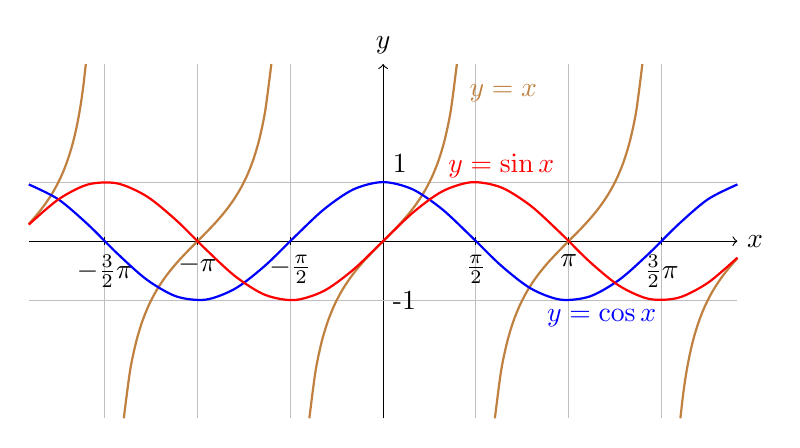
\begin{tikzpicture}[scale=0.75]
  \draw[->] (-6,0) -- (6,0) node[right] {$x$};
  \draw[->] (0,-3) -- (0,3) node[above] {$y$};
  \foreach \x/\xtext in
    {{pi/2}/{\frac \pi 2}, {pi}/{\pi}, {3*pi/2}/{\frac{3}{2}\pi},
    {-pi/2}/{-\frac \pi 2}, {-pi}/{-\pi}, {-3*pi/2}/{-\frac{3}{2}\pi}} {
    \draw[shift={(\x,0)},lightgray] (0,-3) -- (0,3);
    \draw[shift={(\x,0)}] (0pt,2pt) -- (0pt,-2pt) node[below] {$\xtext$};
  }
  \foreach \y in {1, -1} {
    \draw[shift={(0,\y)},lightgray] (-6,0) -- (6,0);
  }
  \draw (0,1) node [above right] {1};
  \draw (0,-1) node [right] {-1};
  \draw[domain=-rad(atan(3)):rad(atan(3)),smooth,variable=\x,brown,thick] plot ({\x},{tan(deg(\x))});
  \draw[domain=pi-rad(atan(3)):pi+rad(atan(3)),smooth,variable=\x,brown,thick] plot ({\x},{tan(deg(\x))});
  \draw[domain=-pi-rad(atan(3)):-pi+rad(atan(3)),smooth,variable=\x,brown,thick] plot ({\x},{tan(deg(\x))});
  \draw[domain=-6:-2*pi+rad(atan(3)),smooth,variable=\x,brown,thick] plot ({\x},{tan(deg(\x))});
  \draw[domain=2*pi-rad(atan(3)):6,smooth,variable=\x,brown,thick] plot ({\x},{tan(deg(\x))});
  \draw[domain=-6:6,smooth,variable=\x,blue,thick] plot ({\x},{cos(deg(\x))});
  \draw[domain=-6:6,smooth,variable=\x,red,thick] plot ({\x},{sin(deg(\x))});
  \draw (3.7,-1) node[blue,below] {$y=\cos x$};
  \draw (2,0.9)  node[red,above] {$y=\sin x$};
  \draw (1.3,2.5) node[brown,right] {$y=\tg x$};
  \end{tikzpicture}
  \caption{%
  I grafici delle funzioni $\sin$, $\cos$ e $\tg$.
  \ifwidemargin\\\\\fi%
  \usebox{\qrfigtrigo}}
\end{figure}

%
\begin{proof}
\mymark{*}
\begin{enumerate}
\item
Essendo $\overline{e^{ix}} = e^{\overline{ix}} = e^{-ix}$
discende dalla formula~\eqref{eq:re_im} per il calcolo
di parte reale ed immaginaria.

\item
Si verifica direttamente con le formule precedenti.

\item
Per $x\in \RR$ si ha da un lato
\[
  \abs{\exp (ix)}^2 = \exp(ix)\cdot \overline{\exp(ix)}
  = \exp(ix)\cdot \exp(-ix)
  = \exp(0) = 1
\]
e dall'altro
\[
  \abs{\exp(ix)}^2 = \abs{\cos x + i \sin x}^2
    = \cos^2 x + \sin^2 x.
\]

\item
Grazie alla formula che esprime l'esponenziale
della somma:
\begin{align*}
\cos(\alpha+\beta) + i \sin(\alpha + \beta)
&= \exp(i(\alpha + \beta))
= \exp(i\alpha) \cdot \exp(i\beta) \\
&= (\cos \alpha + i \sin \alpha) \cdot (\cos \beta + i \sin \beta)\\
&= \cos \alpha \cos \beta - \sin \alpha \sin \beta \\
&\quad + i (\sin \alpha \cos \beta + \cos \alpha \sin \beta)
\end{align*}
e uguagliando parte reale e parte immaginaria si ottengono le formule
di addizione.

\item
Visto che la funzione $\exp\colon \CC \to \CC$ è continua
anche la sua restrizione all'asse immaginario lo è.
E dunque anche parte reale (coseno) e parte immaginaria (seno) lo sono.

\item
Sia $x\in \RR$.
Osservando che $i^{2k} = (i^2)^k = (-1)^k$ e $i^{2k+1}= i \cdot i^{2k}
= i\cdot(-1)^k$ suddividendo i termini pari e dispari
della serie che definisce l'esponenziale si ha:
\begin{align*}
  \exp(ix)
  &= \sum_{k=0}^{+\infty} \frac{i^k x^k}{k!}
  = \sum_{k=0}^{+\infty}\frac{i^{2k} x^{2k}}{(2k)!}
    + \sum_{k=0}^{+\infty}\frac{i^{2k+1} x^{2k+1}}{(2k+1)!}\\
  &= \sum_{k=0}^{+\infty}\frac{(-1)^k x^{2k}}{(2k)!}
    +  i \sum_{k=0}^{+\infty}\frac{(-1)^k x^{2k+1}}{(2k+1)!}.
\end{align*}
Osserviamo ora che le due serie che compaiono a destra dell'uguaglianza
sono a termini reali e quindi la loro somma è reale.
Dunque queste due serie coincidono con la parte reale e la parte immaginaria di $\exp(ix) = \cos x + i \sin x$.

\item
Per la corrispondente proprietà dell'esponenziale
sappiamo che per $x \to 0$ si ha
\[
  \frac{e^{i x}-1}{i x} \to 1.
\]
Ma
\[
  \frac{e^{ix}-1}{i x}
  = \frac{\cos x - 1 + i \sin x}{i x}
  = \frac{\sin x}{x} + i\frac{1- \cos x}{x}.
\]
Scopriamo dunque che
\[
  \frac{1-\cos x}{x} \to 0
  \qquad\text{e}\qquad
  \frac{\sin x}{x} \to 1.
\]
D'altra parte si ha
\begin{align*}
  \frac{1-\cos x}{x^2}
  &=\frac{(1-\cos x)\cdot(1+\cos x)}{x^2(1+\cos x)}
  = \frac{1-\cos^2 x}{x^2} \cdot \frac{1}{1+\cos x}\\
  &= \enclose{\frac{\sin x}{x}}^2\cdot \frac 1{1+\cos x}
  \to 1 \cdot \frac 1 {1+\cos 0} = \frac 1 2.
\end{align*}

\end{enumerate}
\end{proof}

Definiamo $\pi$ come la misura in radianti dell'angolo piatto, 
cioè dell'angolo identificato dal numero $e^{i\pi} = -1$ 
sul piano complesso.

\begin{theorem}[definizione di $\pi$]
\index{$\pi$!definizione}%
\index{$\tau$!definizione}%
\label{th:pi}%
\mynote{$\pi$}%
Definiamo $\pi$ come il più piccolo numero reale
positivo in cui si annulla la funzione $\sin x$.
Si ha $\pi \in [2.8,4]$.
Le funzioni $e^{ix}$, $\sin x$ e $\cos x$ sono
periodiche di periodo $\tau = 2\pi$:
\mynote{$\tau$}%
\[
  e^{i(x+2\pi)} = e^{ix}, \qquad
  \cos(x + 2\pi) = \cos x, \qquad
  \sin(x + 2\pi) = \sin x.
\]
La funzione $\sin x$ è strettamente crescente nell'intervallo
$\closeinterval{-\frac \pi 2}{\frac \pi 2}$
mentre la funzione $\cos x$ è strettamente decrescente 
nell'intervallo $\closeinterval{0}{\pi}$.
Si ha infine:
\begin{align*}
\sin(\pi + x) = -\sin x, \qquad 
\cos(\pi + x) = -\cos x.
\end{align*}

Vale inoltre la celeberrima formula di Eulero:
\index{Eulero!formula di}%
\index{formula!di Eulero}%
\[
  e^{i\pi} + 1 = 0.
\]
\end{theorem}
%%
%%
\begin{proof}
Il teorema~\ref{th:approx_exp} ci permette di approssimare la 
funzione esponenziale $e^{ix}$ per $x\in [0,1]$. 
Ci proponiamo quindi di determinare l'andamento delle funzioni 
$\sin x$ e $\cos x$ in tale intervallo e definire in tale intervallo 
il valore di $\alpha=\frac \pi 4$.
Tramite tale valore $\alpha$ e tramite le formule di addizione riusciremo 
a determinare l'andamento delle funzioni $\sin$ e $\cos$ su tutta la 
retta reale.

Se $x\in[0,1]$ grazie al teorema~\ref{th:approx_exp} applicato 
con $n=3$ sappiamo che 
\begin{align*}
  \abs{e^{ix} - \enclose{1 + ix  + \frac{(ix)^2}{2} + \frac{(ix)^3}{6}}}
  \le \frac{\abs{ix}^4}{18}
\end{align*}
sviluppando
\begin{align*}
  \abs{\cos x + i \sin x - 1 - ix + \frac{x^2}{2} + i\frac{x^3}{6}}
  \le \frac{x^4}{18}.
\end{align*}
Il valore assoluto delle parti reale e immaginaria di un numero 
complesso sono minori del modulo del numero complesso.
Dunque si ottiene:
\begin{align}\label{eq:86035}
    \abs{\cos x - 1 + \frac{x^2}{2}} \le \frac{x^4}{18}\smallskip
    \qquad\text{e}\qquad
    \abs{\sin x - x + \frac{x^3}{6}} \le \frac{x^4}{18}.
\end{align}
Per la funzione $\sin x$ si ha dunque
\begin{align*}
    x - \frac{x^3}{6} - \frac{x^4}{18}
    \le \sin x 
    \le x - \frac{x^3}{6} + \frac{x^4}{18}
\end{align*}
e sapendo che $0<x<1$ possiamo affermare che 
\[
  x - \frac{x^3}{6} - \frac{x^4}{18}
  \ge x - \frac{x}{6} - \frac{x}{18}
  = \frac{7}{9} x
\]
e 
\[
  x - \frac{x^3}{6} + \frac{x^4}{18}
  \le x - \frac{x^3}{6} + \frac{x^3}{18}
  \le x.
\]
Dunque se $x\in[0,1]$ si ha 
\begin{equation}\label{eq:4757614}
  \frac{7}{9} x \le \sin x \le x.
\end{equation}
Per il coseno da un lato osserviamo che da~\eqref{eq:86035}
si ottiene, se $x\in [0,1]$:
\[
\cos x 
  \ge 1 - \frac{x^2}{2} -\frac{x^4}{18}   
  \ge 1 - \frac{1}{2} - \frac{1}{18}
  = \frac 4 9 > 0.
\]
Dall'altro lato si ha
\[
\cos x 
\le 1 - \frac{x^2}{2} + \frac{x^4}{18}
= 1 - \frac{x^2}{2} + \frac{x^2}{18}
\le 1 - \frac{4}{9} x^2.
\]

Vogliamo ora dimostrare che la funzione $\cos x$ 
è strettamente decrescente sull'intervallo $[0,1]$.
Infatti se $x\in[0,1]$ e $t\in(0,1]$ si ha 
\begin{align*}
  \cos(x+t) 
  = \cos x \cos t - \sin x \sin t
  \le \cos x \cos t < \cos x
\end{align*}
in quanto $\sin x\ge 0$, $\sin t \ge 0$ 
e $\cos t < 1 - \frac{5}{9}t^2 < 1$ se $t>0$.
Dunque la funzione $\cos x$ è strettamente 
decrescente su $[0,1]$. 
Visto che $\cos^2 x + \sin^2 x = 1$ 
deduciamo che la funzione $\sin^2 x$ 
è strettamente crescente in $[0,1]$.
Inoltre $\sin x$ è positiva su tale 
intervallo e dunque anche $\sin x$
è strettamente crescente in $[0,1]$.

Vogliamo ora dimostrare che esiste 
$\alpha \in [0,1]$ tale per cui 
$\sin \alpha = \frac{\sqrt 2}{2}$.
Visto che $\sin x$ è una funzione continua, 
e $\sin 0 = 0$, per utilizzare 
il teorema~\ref{th:zeri} dei valori intermedi 
basterà verificare che $\sin 1 > \frac{\sqrt 2}{2}$.
E infatti si ha:
\[
\sin 1 \ge \frac 7 9 > \frac{\sqrt 2}{2}.
\]
Dunque esiste un unico $\alpha\in [0,1]$ 
tale che $\sin \alpha = \frac{\sqrt 2}{2}$.
Allora anche $\cos \alpha = \frac{\sqrt 2}{2}$ 
(in quanto $\sin^2 + \cos^2 = 1$)
e quindi
\[
  e^{2i\alpha} 
  = \enclose{\frac{\sqrt 2}{2} \enclose{1+i}}^2
  = \frac 1 2 \enclose{1+2i-1} = i.
\]
Dunque $\alpha$ è la misura in radianti di metà 
angolo retto.

Se poniamo $\pi = 4\alpha$ scopriamo dunque che 
\[
  e^{i\pi} 
  = \enclose{e^{2i\alpha}}^2
  = i^2 = -1
\]
da cui $\sin \pi = 0$ e $\cos \pi = -1$.
Analogamente da $e^{2i\alpha}=i$ 
troviamo che $\sin \frac \pi 2 = 1$
$\cos \frac \pi 2 = 0$.

Dalla stima~\eqref{eq:4757614} si ottiene 
\[
  \frac 7 9 \alpha 
  \le \frac{\sqrt 2}{2}
  \le \alpha
\]
da cui $\pi=4\alpha \in [2.8, 4]$.

Abbiamo verificato che sull'intervallo 
$\closeinterval{0}{\frac \pi 4}$ la funzione $\sin x$ è strettamente 
crescente mentre $\cos x$ è strettamente decrescente.
Dalle formule di addizione possiamo quindi dedurre che 
$\sin\enclose{\frac \pi 2 - x} = \cos x$ 
e $\cos\enclose{\frac \pi 2 -x} = \sin x$.
Dunque anche sull'intervallo $\closeinterval{\frac \pi 4}{\frac \pi 2}$ 
la funzione $\sin x$ è crescente e $\cos x$ è decrescente.
Ancora, tramite le formula di addizione troviamo che 
$\sin(\pi - x)=\sin x$ e $\cos(\pi - x) = -\cos x$ 
da cui possiamo dedurre che sia la funzione $\sin x$ 
che la funzione $\cos x$ sono strettamente decrescenti 
sull'intervallo $\closeopeninterval{\frac \pi 2}{\pi}$.
Possiamo dunque affermare che $\sin x>0$ se $0<x<\pi$ 
e dunque $\pi$ è il più piccolo reale positivo in cui 
la funzione $\sin$ si annulla.

Visto che $\sin(\pi+x) = -\sin x$ e $\cos(\pi+x)=-\cos x$
possiamo stabilire l'andamento delle funzioni $\sin$ e $\cos$
anche sull'intervallo $\closeinterval{\pi}{2\pi}$.
Infine essendo $e^{2i\pi} = 1$ si osserva che la funzione 
$e^{2ix}$ e di conseguenza le funzioni $\sin x$ e $\cos x$
sono periodiche di periodo $2\pi$.
\end{proof}

\begin{exercise}
  Utilizzando il teorema~\ref{th:approx_e} dimostrare che
  \[
  \lim_{n\to +\infty} n \sin(2\pi e\, n!) = 2\pi.
  \]
\end{exercise}

%%%%
%%%%
%%%%

\section{funzioni trigonometriche inverse}
La funzione $\sin\colon[-\pi/2,\pi/2]\to [-1,1]$ risulta essere strettamente crescente. Inoltre essendo una funzione continua e visto che $\sin(-\pi/2)=-1$
e $\sin(\pi/2) = 1$ per il  teorema dei valori intermedi
la funzione assume tutti i valori in $[-1,1]$.
Dunque restringendo il dominio all'intervallo $[-\pi/2, \pi/2]$
e il codominio all'intervallo $[-1,1]$ la funzione risulta invertibile.
La funzione inversa
\[
  \arcsin\colon[-1,1]\to [-\pi/2, \pi/2]
\]
si chiama \emph{arco seno}. Per definizione di funzione inversa si ha
\[
  \arcsin(\sin x) = x, \qquad \forall x \in [-\pi/2, \pi/2]
\]
e
\[
  \sin(\arcsin x) = x, \qquad \forall x \in [-1, 1].
\]

La funzione $\cos \colon[0,\pi] \to [-1,1]$ risulta essere strettamente
decrescente e, analogamente a quanto visto per la funzione $\sin$
possiamo verificare che ristretta a tali intervalli è una funzione invertibile.
La funzione inversa
\[
  \arccos\colon[-1,1] \to [0,\pi]
\]
si chiama \emph{arco coseno}. Per definizione si ha
\[
  \arccos(\cos x) = x, \qquad \forall x \in [0,\pi]
\]
e
\[
    \cos(\arccos x) = x, \qquad \forall x \in [-1,1].
\]

La funzione
\index{tangente!funzione trigonometrica}
\mymargin{$\tg x$}
\[
\tg x = \frac{\sin x}{\cos x}
\]
è definita quando $\cos x\neq 0$ ovvero:
\[
  \tg \colon \RR \setminus\ENCLOSE{\frac \pi 2+ k\pi\colon k\in \ZZ} \to \RR.
\]
Se restringiamo la funzione all'intervallo $\enclose{-\pi/2, \pi/2}$ possiamo
facilmente osservare che la funzione $\tg\colon(-\pi/2,\pi/2)\to \RR$ è strettamente crescente. Inoltre se $a_n \to \pi/2$, $a_n<\pi/2$ si ha $\cos(a_n)\to 0$ (per continuità del coseno) e $\sin(a_n)\to 1$ dunque $\tg a_n\to +\infty$. Analogamente per $a_n \to -\pi/2$ si trova $\tg a_n \to -\infty$. Dunque per il teorema dei valori intermedi possiamo affermare che la funzione $\tg\colon(-\pi/2,\pi/2)\to \RR$ è suriettiva. E' quindi invertibile
e la funzione inversa
\[
  \arctg \colon \RR \to (-\pi/2,\pi/2)
\]
si chiama \emph{arco tangente}. Per definizione si ha
\[
  \arctg \tg x = x, \qquad \forall x \in (-\pi/2, \pi/2)
\]
e
\[
  \tg\arctg x = x, \qquad \forall x \in \RR.
\]

Grazie al teorema~\ref{th:monotona_continua}%
visto che quest funzioni sono monotone e bigettive
possiamo affermare che
le funzioni $\arcsin$, $\arccos$ e $\arctg$ sono funzioni continue.

\begin{exercise}
Dimostrare che per ogni $x>0$ si ha
\[
  \arctg \frac 1 x = \frac \pi 2 - \arctg x.
\]
\end{exercise}

\begin{exercise}
La serie
\[
  \sum_{k=1}^{+\infty} \frac{\sin k}{k}
\]
è convergente.
\end{exercise}
\begin{proof}
Applichiamo il teorema~\ref{th:dirichlet}.
Posto $a_k = \sin k$ e $B_k=1/k$
si ha
\[
  A_n = \sum_{k=0}^{n-1} \sin k = \Im \sum_{k=0}^{n-1} e^{ik}.
\]
Osserviamo allora che $e^{ik}=(e^i)^k$ e dunque $A_n$ è la parte immaginaria
della somma di una serie geometrica. 
Si può quindi calcolare esplicitamente
\[
  A_n = \Im \frac{1-(e^i)^n}{1-e^i}
\]
da cui
\[
  \abs{A_n} \le \abs{\frac{1-e^{in}}{1-e^i}} \le \frac{1+\abs{e^{in}}}{\abs{1-e^i}}
  = \frac{2}{\abs{1-e^i}}
\]
e dunque $A_n$ è limitata.

D'altro canto posto $B_k = 1/k$ è chiaro che $B_k$ è
decrescente e infinitesima.
\end{proof}

\begin{exercise}
Determinare il carattere delle seguenti serie
\[
  \sum_n \enclose{\frac 1 n - \sin \frac 1 n},\qquad
  \sum_n \sin\enclose{\pi n + \frac 1 n}
\]
\end{exercise}

\section{funzioni iperboliche}

\begin{definition}[funzioni iperboliche]
Le funzioni
\emph{coseno iperbolico} e \emph{seno iperbolico}
sono definite, per ogni $x\in \RR$,
come segue:
\mymargin{$\sinh$, $\cosh$}%
\index{funzioni!iperboliche}%
\index{seno!iperbolico}%
\index{coseno!iperbolico}%
\index{$\sinh$}%
\index{$\cosh$}%
\begin{equation}
\label{eq:sinh_cosh}
  \cosh x = \frac{e^x + e^{-x}}{2},
  \qquad
  \sinh x = \frac{e^x - e^{-x}}{2}.
\end{equation}
\end{definition}

\begin{theorem}[proprietà delle funzioni iperboliche]
Valgono le seguenti proprietà.
\begin{enumerate}
\item
la funzione $\sinh$ è dispari, $\cosh$ è pari:
\[
\sinh(-x) = -\sinh(x),
\qquad
\cosh(-x) = \cosh(x);
\]

\item
i punti del piano con coordinate $(\cosh x, \sinh x)$
per $x\in \RR$
sono disposti su un ramo di iperbole in quanto vale:
\[
  \cosh^2 x - \sinh^2 x = 1;
\]

\item formule di addizione:
\begin{align*}
  \cosh(\alpha+\beta) &= \cosh \alpha \cosh \beta + \sinh \alpha \sinh \beta,\\
  \sinh(\alpha+\beta) &= \sinh \alpha \cosh \beta + \cosh \alpha \sinh \beta;
\end{align*}

\item si ha
\begin{align*}
  \cosh x
  &= \sum_{k=0}^{+\infty} \frac{x^{2k}}{(2k)!}
  = 1 + \frac{x^2}{2} + \frac{x^4}{4!} + \frac{x^6}{6!} + \dots \\
  \sinh x
  &= \sum_{k=0}^{+\infty} \frac{x^{2k+1}}{(2k+1)!}
  = x + \frac{x^3}{6} + \frac{x^5}{5!} + \frac{x^7}{7!} + \dots
\end{align*}

\item
la funzione $\sinh$ è strettamente crescente su tutto $\RR$,
la funzione $\cosh$
è strettamente crescente sull'intervallo
$[0,+\infty)$ e strettamente decrescente
nell'intervallo $(-\infty,0]$;

\item per $x\to +\infty$ si ha $\sinh x \to +\infty$, $\cosh x \to +\infty$, 
per $x\to -\infty$ si ha $\sinh x \to -\infty$, $\cosh x \to +\infty$.

\end{enumerate}
\end{theorem}

\newsavebox{\qrfigiperb}\sbox{\qrfigiperb}{\myurlhere{figiperb}{funzioni iperboliche}}%
\begin{figure}
  \centering%
  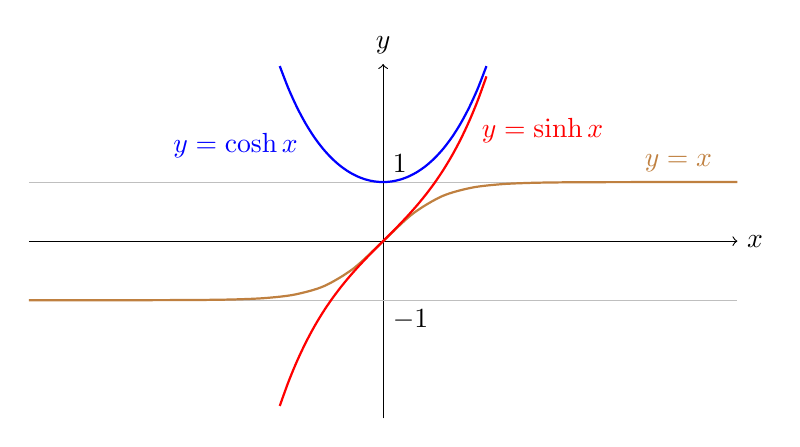
\begin{tikzpicture}[scale=0.75]
  \draw[->] (-6,0) -- (6,0) node[right] {$x$};
  \draw[->] (0,-3) -- (0,3) node[above] {$y$};
  \foreach \y in {1, -1} {
    \draw[shift={(0,\y)},lightgray] (-6,0) -- (6,0);
  }
  \draw (0,1) node [above right] {$1$};
  \draw (0,-1) node [below right] {$-1$};
  \draw[domain=-6:6,smooth,variable=\x,brown,thick] plot ({\x},{tanh(\x)});
  \draw[domain=-1.75:1.75,smooth,variable=\x,blue,thick] plot ({\x},{cosh(\x)});
  \draw[domain=-1.75:1.75,smooth,variable=\x,red,thick] plot ({\x},{sinh(\x)});
  \draw (-2.5,2) node[blue,below] {$y=\cosh x$};
  \draw (2.7,1.5)  node[red,above] {$y=\sinh x$};
  \draw (5,1) node[brown,above] {$y=\tgh x$};
  \end{tikzpicture}
  \caption{%
    I grafici delle funzioni $\sinh$, $\cosh$ e $\tgh$.
    \ifwidemargin\\\\\fi%
    \usebox{\qrfigiperb}%
  }
\end{figure}

\begin{proof}
I primi tre punti si dimostrano facilmente per verifica diretta,
utilizzando la definizione~\eqref{eq:sinh_cosh}.

Gli sviluppi in serie si ottengono anch'essi sostituendo
gli sviluppi dell'esponenziale nella definizione.
Nel $\cosh$ i termini di grado dispari si cancellano, nel $\sinh$ si cancellano
i termini di grado pari.

Per quanto riguarda la monotonia si osserva che se $x\ge 0$ ogni
addendo delle due serie esposte nel punto 4 è strettamente crescente
(in quanto i coefficienti sono tutti positivi) e dunque le somme delle serie,
cioè la funzione $\cosh$ e la funzione $\sinh$ sono strettamente crescenti
sull'intervallo $[0,+\infty)$. La funzione $\sinh$, essendo dispari,
risulta inoltre crescente anche sull'intervallo $(-\infty,0]$ e quindi
è crescente su tutto $\RR$.

Per l'ultima proprietà basterà usare la definizione~\eqref{eq:sinh_cosh}
e ricordare che (teorema~\ref{th:ordine_infinito})
se $x\to +\infty$ allora
$e^x\to +\infty$ ed $e^{-x}=\frac{1}{e^{x}} \to 0$.
\end{proof}

Osserviamo che $\cosh 0 = 1$ e, per le proprietà di monotonia viste nel teorema
precedente si ha $\cosh x \ge \cosh 0 = 1 > 0$. Dunque $\cosh x$ non si annulla
mai e si può definire per ogni $x\in \RR$ la \emph{tangente iperbolica}
\index{tangente!iperbolica}%
\mymargin{$\tgh$}%
\[
    \tgh x = \frac{\sinh x}{\cosh x}.
\]

La funzione $\sinh\colon \RR\to\RR$ è iniettiva in quanto strettamente crescente ed
è surgettiva in quanto è continua e quindi assume tutti i valori compresi tra
$\lim_{x\to+\infty} \sinh(x) = +\infty$ e $\lim_{x\to -\infty} \sinh(x) = -\infty$. 
Dunque $\sinh\colon \RR \to \RR$
è invertibile e la funzione inversa si chiama \emph{settore di seno iperbolico}
e si denota con
\mymargin{$\settsinh$}
\index{settore!di seno iperbolico}
\[
    \settsinh \colon \RR \to \RR.
\]
Analogamente la funzione ristretta $\cosh\colon [0,+\infty)\to [1,+\infty)$ è
iniettiva in quanto strettamente crescente ed è surgettiva in quanto
è continua e assume su $[0,+\infty)$ tutti i valori compresi tra $\cosh(0)=1$ e
$\lim_{x\to +\infty} \cosh x = +\infty$.
Dunque la funzione $\cosh x$ ristretta a $[0,+\infty)\to [1,+\infty)$
è invertibile e la funzione inversa si chiama \emph{settore di coseno iperbolico}
\mymargin{$\settcosh$}
\index{settore!di coseno iperbolico}
\[
    \settcosh \colon [1,+\infty)\to [0,+\infty).
\]

La funzione $\tgh x$ è strettamente crescente su tutto $\RR$ e assume tutti i valori strettamente compresi tra $-1$ e $1$.
La funzione inversa si chiama $\setttgh$.

\begin{exercise}
Fissato $y\in \RR$ si risolva l'equazione
\[
    \frac{e^x - e^{-x}}{2} = y
\]
riconducendola ad una equazione di secondo grado nella variabile $t=e^x$.
Si dimostri quindi che vale
\[
    \settsinh x = \ln\enclose{x + \sqrt{x^2 + 1}}.
\]
In modo analogo si dimostri che vale
\[
    \settcosh x = \ln\enclose{x + \sqrt{x^2 - 1}}
\]
e
\[
    \setttgh x = \ln \sqrt{\frac{1+x}{1-x}}.
\]
\end{exercise}


\section{esercizi}
\begin{exercise}
Determinare il carattere delle seguenti serie
\[
    \sum_n \frac{n^2-n^3}{3^n}, \qquad
    \sum_n \frac{(n!)^2}{(2n)!}
\]
\[
\sum_n \frac{(-1)^n}{\ln\abs{n^7 - 10n^5 + 3}},  \qquad
\sum_n \frac{n-10}{n^2+10}
\]
\end{exercise}
  